% !TEX root = ../../thesis.tex

\newpage
\vphantom{}
\section{Beyond the leading order}
Deriving the wave kinetic equation by truncating perturbation theory at higher orders is not an easy feat. Calculations become quickly extremely cumbersome. Approaches 
based on classical diagrammatic methods were developed in \cite{Zakharov1975} and \cite{Gurarie:1994ut}. Lately techniques exploiting Feynman diagrams were developed in
\cite{Rosenhaus2023}, \cite{Rosenhaus:2022uwa} and \cite{Rosenhaus:2023sik}. This new methods allow for a relatively fast derivation of higher order kinetic equations.
Such equations and their validity are discussed in \cite{Rosenhaus:2023pdj}. The possibility of gaining insight into the strong turbulent regime by resumming 
part of the corrections was investigated instead in \cite{Rosenhaus:2025mgj}. \\
The focus of this chapter is to introduce the computational tools to consistently derive kinetic equations with contributions from higher powers of the coupling. 
The methods of \cite{Rosenhaus2023} are discussed in a generic four wave system. First we show \hl{MAYBE CITE SIGGIA ROSEN MARTIN} how to map the derivation of the kinetic equation into
the task of evaluating correlators in a Quantum Field Theory model. The basic idea is that a nonlinear system coupled to a random forcing may be regarded as 
a statistical theory were the normal variables of the orginal system inherit the stochastic properties of the forcing. If the system spectrum in Fourier space is continous
a path integral approach may be implemented, allowing for the usage of the well developed machinery of QFT perturbation theory.\\
After introducing and commenting the Feynman rules of the model, we calculate two and four points 
correlation functions up to the first nontrivial higher order to derive the corresponding kinetic equation. The resulting theory can be said to account 
not only for direct four wave interactions,as \eqref{kinetic}, but also for the exchange of virtual waves among different modes. We end the chapter by briefly discussing the implications
of this corrected equations for the KZ spectra. \\  
\subsection{Path integral formulation of weak turbulence theory}

There are many ways to derive the kinetic equation for weakly interactive waves. One of them is by looking at the late time behaviour of the same nonlinear system
coupled to a complex gaussian forcing and some dissipation, as in \cite{Zakharov1975} we write the modified e.o.m.s (already in the continuum limit)
\begin{equation}
    \pt a_k + i \omga_k a_k = -i \sum_{123}\Tint_{k123} \aonestar\atwo\athree \delta^{k1}_{23} + f_k(t) - \gamma_k a_k
    \label{eoms}
\end{equation}

and impose guassian statistics on the forcing
\begin{equation}
    \langle f_k(t)f_p(t')\rangle = \F_k \delta(k-p)\delta(t-t').
\end{equation}
solving the system perturbatively and looking at a big enough $t$, equation \eqref{kinetic} is recovered. \\
The forcing and dissipation introduced this way are not of physical importance and have nothing to do with the $\Gamma_k$ term responsible 
for the energy and wave action cascades. The contribution of $f_k$ is to introduce randomness into the system, in place of the explicit RPA assumption. 
The last step of the derivation then removes this nonphysical elements by taking the limit of both $\F_k$ and $\gamma_k$ to zero, while keeping their ratio finite as
to obtain a finite wave density $n_k$. \\  
\hl{SCRIVI CONTO SE C'E' TEMPO} \\
This is the starting point adopted by Rosenhaus and Smolkin in \cite{Rosenhaus2023} to access, with manageable calculation, higher orders in perturbation theory. We will 
follow their method in this section.\\
The basic idea is to reformulate the theory in the language of path integrals, to then move the statistics from the forcing to the canonical variables $\ak$. We start by
explicitly writing the probability distribution for a given $f_k(t)$ functional form as 
\begin{equation}  
    \mathrm{P}[f] \sim e^{-\int dt \sum_k \frac{|f_k(t)|^2}{\F_k}},
\end{equation}
Where instead of an integration on $k$, even if we are in the continuum limit, we write a sum. This choice is to improve clarity in the cumbersome formulas 
we will later write, but sums should always be intended as integrals. We write the expectation value of a general composition of variables $O(a)$ \footnote{
    In general it could be the composition of various $\ak = ak(t)$ at different wave numbers and different times.
} as 
\begin{equation}
    \langle O(a) \rangle = \frac{1}{\mathrm{Z}}\int \D f \D f^* \mathrm{P}[f] O(a), 
\end{equation}
where the integration measure $\D f$ is a formal sum over all possible functions $f_k(t) = f(k,t)$ and $\mathrm{Z}$ is a normalization constant. If $k$ and $t$ instead of continous variables were discrete labels $i$ and $j$,
the integration measure would be the product $\prod_{ij}d f_{ij}$, running over all the possible values of the labels. \\
We want the $a$ variables to satisfy the equations of motion, we may impose so by first defining a function $\Ef$ as
\begin{equation}
    \Ef = \pt a_k + i \omga_k a_k +i \sum_{123}\Tint_{k123} \aonestar\atwo\athree \delta^{k1}_{23} - f_k(t) + \gamma_k a_k,
    \label{Eeffe}
\end{equation}  
so that the requirement that $\ak$ is a solution of the e.o.m.s may be expressed through a functional $\delta$ imposing $\Ef = 0$. We also need to add an integration measure
$\D \Ef \D \Efstar$ to guarantee the normalization of the probability distribution. The result for a generical expectation value is
\begin{equation}
    \langle O(a) \rangle = \frac{1}{\mathrm{Z}}\int \D f \D f^* \D \Ef \D \Efstar \mathrm{P}[f] O(a)\delta(\Ef)\delta(\Efstar).
\end{equation} 
It is important to notice that we are explicitely writing a measure for a variable and another for its complex conjugate. It is customary that each functional integration
represents an infinity of ordinary integrations of the same cardinality of a line. Thus complex variables require a double measure each\footnote{We formally use a variable 
and its conjugate instead of its real and imaginary part in the same way as one can formally describe the complex plane by using $z$ and $z^*$ instead of x and y.}.\\
\begin{comment}
To ease the upcoming computation we perform the change of variables 
\begin{equation}
    \left(\Ef,\Efstar\right)\rightarrow \left( \text{Re}\{Ef\},\text{Im}\{\Ef\} \right),
\end{equation}
that obviously has a unitary Jacobian\footnote{It consists in an infinite set of transformations $(z, z^*)\rightarrow (x,y)$.}
\end{comment}
Given that we desire a theory where the dynamical variables are the $a$s, we perform a change of coordinates from $\left(\Ef,\Efstar \right)$
to $\left( \anorm, \astar\right)$, resulting in 
\begin{equation}
    \langle O(a) \rangle = \frac{1}{\mathrm{Z}}\int \D f \D f^* \D \anorm \D\astar  \mathrm{P}[f] O(a)\delta(\Ef)\delta(\Efstar)
    \left| \frac{\partial \left( \Ef,\Efstar\right)}{\partial \left( \anorm, \astar\right)}\right|.
    \label{expect1}
\end{equation}
The Jacobian has to interpreted as the matrix 
\begin{equation}
     \frac{\partial \left( \Ef,\Efstar\right)}{\partial \left( \anorm, \astar\right)} = 
    \renewcommand{\arraystretch}{1.8}  % Aumenta la distanza verticale
    \setlength{\arraycolsep}{6pt}     % Aumenta la distanza orizzontale
    \begin{pmatrix}
        \frac{\partial \Ef}{\partial \anorm}  & \frac{\partial \Efstar}{\partial \anorm} \\
        \frac{\partial \Ef}{\partial \astar}  & \frac{\partial \Efstar}{\partial \astar}
    \end{pmatrix}
,
\label{Jacobian}
\end{equation}
where each component is in turn a matrix with infinitely many rows and columns\footnote{We are again interpreting a function as a vector with infinite elements.}. \\
Thanks to Sylvester's formula we know that 
\begin{equation}
    \renewcommand{\arraystretch}{1.8}  % Aumenta la distanza verticale
    \setlength{\arraycolsep}{6pt}     % Aumenta la distanza orizzontale
    \left|
    \begin{pmatrix}
        \frac{\partial \Ef}{\partial \anorm}  & \frac{\partial \Efstar}{\partial \anorm} \\
        \frac{\partial \Ef}{\partial \astar}  & \frac{\partial \Efstar}{\partial \astar}
    \end{pmatrix}
    \right|
    = \left| \frac{\partial \Ef}{\partial \anorm} \frac{\partial \Efstar}{\partial \astar} - \frac{\partial \Efstar}{\partial \anorm} 
    \frac{\partial \Ef}{\partial \astar}\right|.
    \label{sylvester}
\end{equation}
To calculate the determinant of the Jacobian we thus have to evaluate the single elements of \eqref{Jacobian}. To do so we first discretize time in \eqref{Eeffe}, obtaining
\begin{equation}
    \Ef (t) \longrightarrow \Delta t \mathrm{E}_f^{i} = a_k^i - a_k^{i-1} + 
    \Delta t\left(i \frac{\delta \Ham}{\delta a_k^{i-1}} - f_k^{i-1} + \gamma_k^{i-1}a_k^{i-1}\right).
    \label{discretization}
\end{equation}
As $\mathrm{E}_i$ does not depend on any $a_k^{j}$ with $j > i$ both the diagonal terms in \eqref{Jacobian} are triangular matrices, moreover the diagonal only contains 
ones as the dependance on $a_k^{i}$ is linear. \\
The remaining elements of the \eqref{Jacobian} are triangular matrices with the diagonal containing only zeroes, as
$\mathrm{E}_f^{i*}$ and  $\mathrm{E}_f^{i}$ do not depend on $a_k^{i}$  and $a_k^{i*}$ respectively. Knowing that the product of such two matrices is null lets us remove it 
from \eqref{sylvester}. \\
Given that the determinant of a triangular matrix is equal to the product of its diagonal elements we find 
\begin{equation}
    \renewcommand{\arraystretch}{1.8}  % Aumenta la distanza verticale
    \setlength{\arraycolsep}{6pt}     % Aumenta la distanza orizzontale
    \left|
    \begin{pmatrix}
        \frac{\partial \Ef}{\partial \anorm}  & \frac{\partial \Efstar}{\partial \anorm} \\
        \frac{\partial \Ef}{\partial \astar}  & \frac{\partial \Efstar}{\partial \astar}
    \end{pmatrix}
    \right|
    = \left| \frac{\partial \Ef}{\partial \anorm} \frac{\partial \Efstar}{\partial \astar}\right|
    = \left| \frac{\partial \Ef}{\partial \anorm} \right| \left|\frac{\partial \Efstar}{\partial \astar}\right|
    = 1,
\end{equation} 
thus letting us remove the Jacobian from \eqref{expect1}.\\
We now use the functional integral representation of $\delta$
\begin{equation}
    \delta(\Ef)\delta(\Efstar) = \int \D \eta\D \eta^* e^{i\int dt \sum_{k}\left( \eta_k^{}\Efstar +\eta_k^* \Ef\right)}
\end{equation}
to obtain 
\begin{equation}
    \langle O(a) \rangle = \frac{1}{\mathrm{Z}}\int \D f \D f^* \D \anorm \D\astar\D \eta\D \eta^*  O(a)
    e^{-\int dt \sum_k \left( \frac{|f_k(t)|^2}{\F_k} - i\eta_k^{}\Efstar -i\eta_k^* \Ef \right)}.
    \label{expect2}
\end{equation}
$\Ef$ only depends on $f_k$ linearly by construction. To integrate out the forcing from the theory we notice that the exponent's part depending on $f_k$
can be reformulated partly as a Gaussian. 
Let us look at the same problem in a simplified setting where $(f_k^{},f_k^*)  \rightarrow (z, z^*)$, $(\eta_k^{}, \eta_k^*) \rightarrow (u, u^*)$ and $\F_k \rightarrow c$.
The part of the exponent under consideration is then
\begin{equation}
    -\frac{zz^*}{c} + iuz^* + iu^*z = -\frac{1}{c} \left(z - iuc \phantom{z^*}\hspace{-3mm}\right)\left(z^* - iu*c \right) - uu^*c,
\end{equation}
where we completed the square. The procedure is easily extendable to the infinite dimensional case. After integrating out the Gaussian integral and absorbing it into the 
normalization constant\footnote{With the difference that there is not a closed form expression 
for the value of the integral, we only now that under a change of coordinates there is a noninteracting free theory. Given that this theory is decoupled 
from the dynamical variables we are interested in,
we can just ignore it. This is what we mean by absorbing it into the normalization constant.}  we find
\begin{equation}
    \langle O(a) \rangle = \frac{1}{\mathrm{Z}}\int\D \anorm \D\astar\D \eta\D \eta^*  O(a)
    e^{-\int dt \sum_k \left( \eta_k^{}\eta_k^* F_k - i\eta_k^{}\Efstarz -i\eta_k^* \Efz \right)},
    \label{expect3}
\end{equation}
where $\Efz$ corresponds to $\Ef$ without forcing term. In an analogous way, by again completing the square, the integral over $\eta$ and $\eta^*$ may be performed and 
absorbed into the normalization constant.
The result is 
\begin{equation}
    \langle O(a) \rangle = \frac{1}{\mathrm{Z}}\int\D \anorm \D\astar O(a)
    e^{-\int dt \Lag},
    \label{expect}
\end{equation} 
with $\Lag$ defined as 
\begin{equation}
    \Lag = \sum_k \frac{|\Efz|^2}{\F_k}.
    \label{Lag}
\end{equation}
What we have found is a statistical theory of the dynamical variables $\anorm$ and $\astar$ in the continuum limit. Through a Wick rotation $t \rightarrow \tau = it$ we 
may turn it into a Quantum Field Theory, where the machinery of Feynman diagrams can be utilized to perform efficient perturbative calculations.\\

\subsection{Feynman rules} 

Our objective is still the kinetic equation. Starting from the original equations of motions \eqref{eoms}, without forcing and dissipation
\begin{equation}
    \pt a_k + i \omga_k a_k = -i \sum_{123}\Tint_{k123} \aonestar\atwo\athree \delta^{k1}_{23},
\end{equation}
multiplying it for $\akstar$ and summing its complex conjugate we obtain
\begin{equation}
    \pt \ak \akstar = -2 \text{Im}\left( \sum_{123}\Tint_{k123}\ak \aone \atwostar \athreestar \delta^{k1}_{34} \right).
\end{equation} 
By averaging over all possible realizations and expliciting the time dependences we find
\begin{equation}
    \pt \langle \ak(t) \akstar(t) \rangle = -2 \text{Im}\left( \sum_{123}\Tint_{k123}\langle\ak(t) \aone (t)\atwostar(t) \athreestar (t)\rangle\delta^{k1}_{34} \right),
    \label{kineticprototype}
\end{equation}
where on the l.h.s. we can see the definition of $n_k(t)$ given in \eqref{wavdef}. We notice from this equation how any order of the kinetic equation can be obtained 
by evaluating four points functions at equal times, togheter with the RPA assumption. Those four points function can be evaluated by the path integral statistical theory 
derived in the last section, where the RPA assumption is recovered through the gaussian statistics over the forcing. Of course we will have to properly 
switch off the contributions form the forcing variance $\F_k$ and the dissipation $\gamma_k$ to obtain results consistent with the first chapter. \\
The good news is that through Feynman diagrams we can calculate four point functions with relative ease. In this section we will write and explain the Feynman rules. 
A full derivation would imply an introduction to Quantum Field Theory, a task out of the scope of this thesis. The reader not familiar with the topic is directed to 
the variety of existing books (for example \cite{Bjorken:1965zz}). \\

We start by expliciting writing $\Lag$ as
\begin{equation}
    \Lag = \sum_k \frac{|\Efz|^2}{\F_k} = \sum_k \frac{1}{\F_k} \left| \pt a_k + i \omga_k a_k + i \sum_{123}\Tint_{k123} \aonestar\atwo\athree \delta^{k1}_{23} \right|^2.
\end{equation} 
Regrouping the different terms order by order $\Lag$ becomes 
\begin{equation}
    \Lag = \Lag_0 + \Lag_1 + \Lag_2.
\end{equation}
with, by extensive usage of the symmetries of $\Tint$ and dummy variables, 
\begin{align}
    \Lag_0 &= \sum_k\frac{1}{\F_k} \left| \Dcov_k a_k  \right|^2, \\
    \Lag_1 &= \frac{i}{2}\sum_{k123}\Tint_{k123}\left( \frac{\Dcovd_k}{\F_k} + \frac{\Dcovd_1}{\F_1} - \frac{\Dcov_2}{\F_2} - \frac{\Dcov_3}{\F_3} \right)
    \akstar \aonestar \atwo \athree, \\
    \Lag_2 &= \sum_{k123456} \frac{1}{\F_k}\Tint_{123k}\Tint_{k456}\aonestar \atwostar \athree \afourstar \afive \asix. 
\end{align}
In this last set of equations we defined 
\begin{equation}
    \Dcov_k a_k = \left(\pt + i\omga_k+ \gamma_k\right)\ak
\end{equation} 
and $\Dcovd_k \akstar$ is its complex conjugate. Moreover in every expression 
like $\frac{\Dcovd_1}{\F_1}\akstar \aonestar \atwo \athree$ the $\Dcovd_k$ always acts only on the normal variable bearing its own argument. \\

We shall directly write the Feynman rules in frequency space, as the calculations are easier this way. We will need to transform back to $t$-space every 
correlator we obtain.\\
Up until now we have been using $\omga_k$ and $\omga_i$ as $\omga(k)$ and $\omga(k_i)$, to avoid introducing unnecessary confusion the 
fourier transform frequency will be named $\omgatt$ . Therefore the fourier transform of a function of $t$ will be a function of $\omgatt$ and the fourier 
transform of a function of $t_i$ will be a function of $\omgatt_i$. \\
The propagator of the free theory may be obtained inverting the quadratic part of the Lagrangian ($\Lag_0$), yealding 
\begin{equation}
    G_{k1}(t_1 - t_2) = \langle \akstar(t_1)\aone(t_2)\rangle = \F_k \delta(k-k_1)\int \frac{d \omgatt}{2\pi}\frac{e^{i\omgatt(t_1 - t_2)}}
    {\left(\omgatt -\omga_k + i\gamma_k \right)\left(\omgatt -\omga_k-i \gamma_k\right)}. 
    \label{propspace}
\end{equation}
It is instructive to look at its explicit form. We use Jordan's lemma to close the integration path in the upward or downward half of the complex plane, obtained by 
making the variable $\omgatt$ complex, depending on the sign of $t_1 - t_2$. We then use the residue theorem to give an explicit form to the propagator, obtaining
\begin{multline}
    G_{k1}(t_1 - t_2) = \langle \akstar(t_1)\aone(t_2)\rangle = \\
    \frac{\F_k}{2\gamma_k}\delta(k-k_1)\left(\theta(t_1-t_2)e^{i(\omga_k + i\gamma_k)(t_1 - t_2)}
    +\theta(t_2-t_1)e^{i(\omga_k - i\gamma_k)(t_1 - t_2)}\right),
\end{multline}  
where $\theta(x-y)$ is the Heavyside's function. Given the definition of the wave action density as an equal time two point correlator, we may conclude that for a 
free theory
\begin{equation}
    n_k = \frac{F_k}{2\gamma_k}.
    \label{freenwav}
\end{equation}
This makes perfectly sense, as in the absence of nonlinear terms there is no exchange of energy among modes, and thus the wave action density at a given $k$ is determined
only by the ratio of the forcing variance (how many waves are introduced at $k$) and the dissipation (how many waves are destroyed at $k$). \\
The Fourier transform of the free theory propagator is
\begin{equation}
    \tilde{G}^0_{k1}(\omga)=\delta(k-k_1)\D^0_k=\delta(k-k_1)\F_k|\G_k|^2,
    \label{prop}
\end{equation}  
where we defined 
\begin{equation}
    \G_j = \frac{i}{\omgatt + i\gamma_j -\omga_j}.
\end{equation}
The full Feynman rules in frequency space are\\
\begin{center}
    \begin{tikzpicture}
    \begin{feynman}
      \vertex[label=left:{\(1\)}] (i) at (-0.75,0);
      \vertex [right=1.5cm of i] (f);
  
      \diagram* {
        (i) -- [fermion, arrow size=1.1pt] (f);
      };
    \end{feynman}
  
     % Arrow pointing to the first equation
    \draw[->] (2,0) -- (3,0);
    % First equation on the right
    \node at (6,0) {\(F_1|\G_1|^2\)};
    \begin{feynman}
      \vertex (v1) at (0,\ytwo);
      \vertex [below left=1cm of v1] (ii4){\(4\)};
      \vertex [below right=1cm of v1] (ii3) {\(3\)};
      \vertex [above left=1cm of v1] (ff1) {\(1\)};
      \vertex [above right=1cm of v1] (ff2) {\(2\)};

      \diagram* {
        (ii4) -- [fermion, arrow size=1.1pt] (v1) -- [fermion, arrow size=1.1pt] (ff1),
        (ii3) -- [fermion, arrow size=1.1pt] (v1) -- [fermion, arrow size=1.1pt] (ff2),
      };
    \end{feynman}

    \draw[->] (2,\ytwo) -- (3,\ytwo);

    \node at (8,\ytwo) {\begin{math}\text{-}i\pi\Tint_{1234}\left(\dfrac{1}{\G_1^*\F_1^{}}+\dfrac{1}{\G_2^*\F_2^{}}-\dfrac{1}{\G_3^{}\F_3^{}}
        -\dfrac{1}{\G_4^{}\F_4^{}}\right)\delta(\delomegatt^{12}_{34})\delta^{12}_{34}\end{math}};
  
    \begin{feynman}
    % Central vertex
      \vertex (center) at (0,\y);

      % Define six external vertices at 60-degree intervals around the center
      \vertex[label=\(2\)] (i2) at ($(center) + (90:1)$);   % 90 degrees (top)
      \vertex[label=left:\(1\)] (i1) at ($(center) + (150:1)$);  % 150 degrees (top-left)
      \vertex[label=left:\(6\)] (f6) at ($(center) + (210:1)$);  % 210 degrees (bottom-left)
      \vertex[label=below:\(5\)] (f5) at ($(center) + (270:1)$);  % 270 degrees (bottom)
      \vertex[label=right:\(4\)] (i4) at ($(center) + (330:1)$);  % 330 degrees (bottom-right)
      \vertex[label=right:\(3\)] (f3) at ($(center) + (30:1)$);   % 30 degrees (top-right)

    % Draw the interactions (lines) between the central vertex and the six external vertices
      \diagram*{
        (i4) -- [fermion, arrow size=1.1pt] (center) -- [fermion, arrow size=1.1pt] (f3),
        (i1) -- [fermion, arrow size=1.1pt] (center) -- [fermion, arrow size=1.1pt] (f6),
        (i2) -- [fermion, arrow size=1.1pt] (center) -- [fermion, arrow size=1.1pt] (f5),
      };
    \end{feynman}

    \draw[->] (2,\y) -- (3,\y);

    \node at (6,\y) {\(\text{-}\sum_{k}\limits\dfrac{\Tint_{123k}\Tint_{k456}}{F_k}2\pi\delta(\delomegatt^{124}_{356})\delta^{12}_{3k}\delta^{k4}_{56}\)};
  
  \end{tikzpicture} 
\end{center}
where $ \delomegatt^{124}_{356} = \omgatt_1 + \omgatt_2 + \omgatt_4 - \omgatt_3 - \omgatt_5 - \omgatt_6$. \\

In the QFT interpretation the deltas over $\omgatt$ and $k_i$ enforce conservation of energy and momentum in any given process. To calculate an $n$-points 
correlation function one has to draw all topologically inequivalent connected diagrams with $n$ external legs, i.e all diagrams that cannot be continously deformed into each other.
Those diagrams may be assembled only through the vertices present in the Feynman rules. To every line composing a diagram a number $i$ is associated,
meaning that every mathematical expression represented by that line is a function of $k_i$ and $\omgatt_i$. Every vertex corresponds to the mathematical expressions 
written above, every external or internal line corresponds to the insertion of a propagator in fourier space $(k, \omgatt)$. For every internal line bearing a number 
$i$, an additional integration $\sum_i \int \frac{d\omgatt_i}{2\pi}$ is to be performed. Additionaly a numerical factor has to be introduced accounting for all the possible 
ways of attaching the external legs to the vertices and external lines obtaining equivalent diagrams. \\
The perturbative order of a given diagram\footnote{Thus also of the mathematical expression it represents.} is equal to $q + 2s$ , where $q$ is the number of quartic vertices 
and $s$ is the number of sextic ones. In the first case only a coupling $\Tint$ appears in the rules and in the second case two of them are present. 
We will now turn to the calculation and analysis of the two and four points functions, in order to obtain a kinetic equation. \\

\subsection{Two points functions}
Let us start by calculating the first order correction to the two points function, the only diagram to consider is the one in figure \ref{fig:oneloop2}. It is made 
of three lines, one of which is internal, and a quartic vertex where $k_3 = k_2$ and $k_1 = k_4$. Given that the number of holes in a diagram grows with the perturbative order, this is usually called a one loop diagram
\footnote{Another common name is NLO contribution, short for next to leading order.}.\\
\begin{figure}[ht]
    \centering
    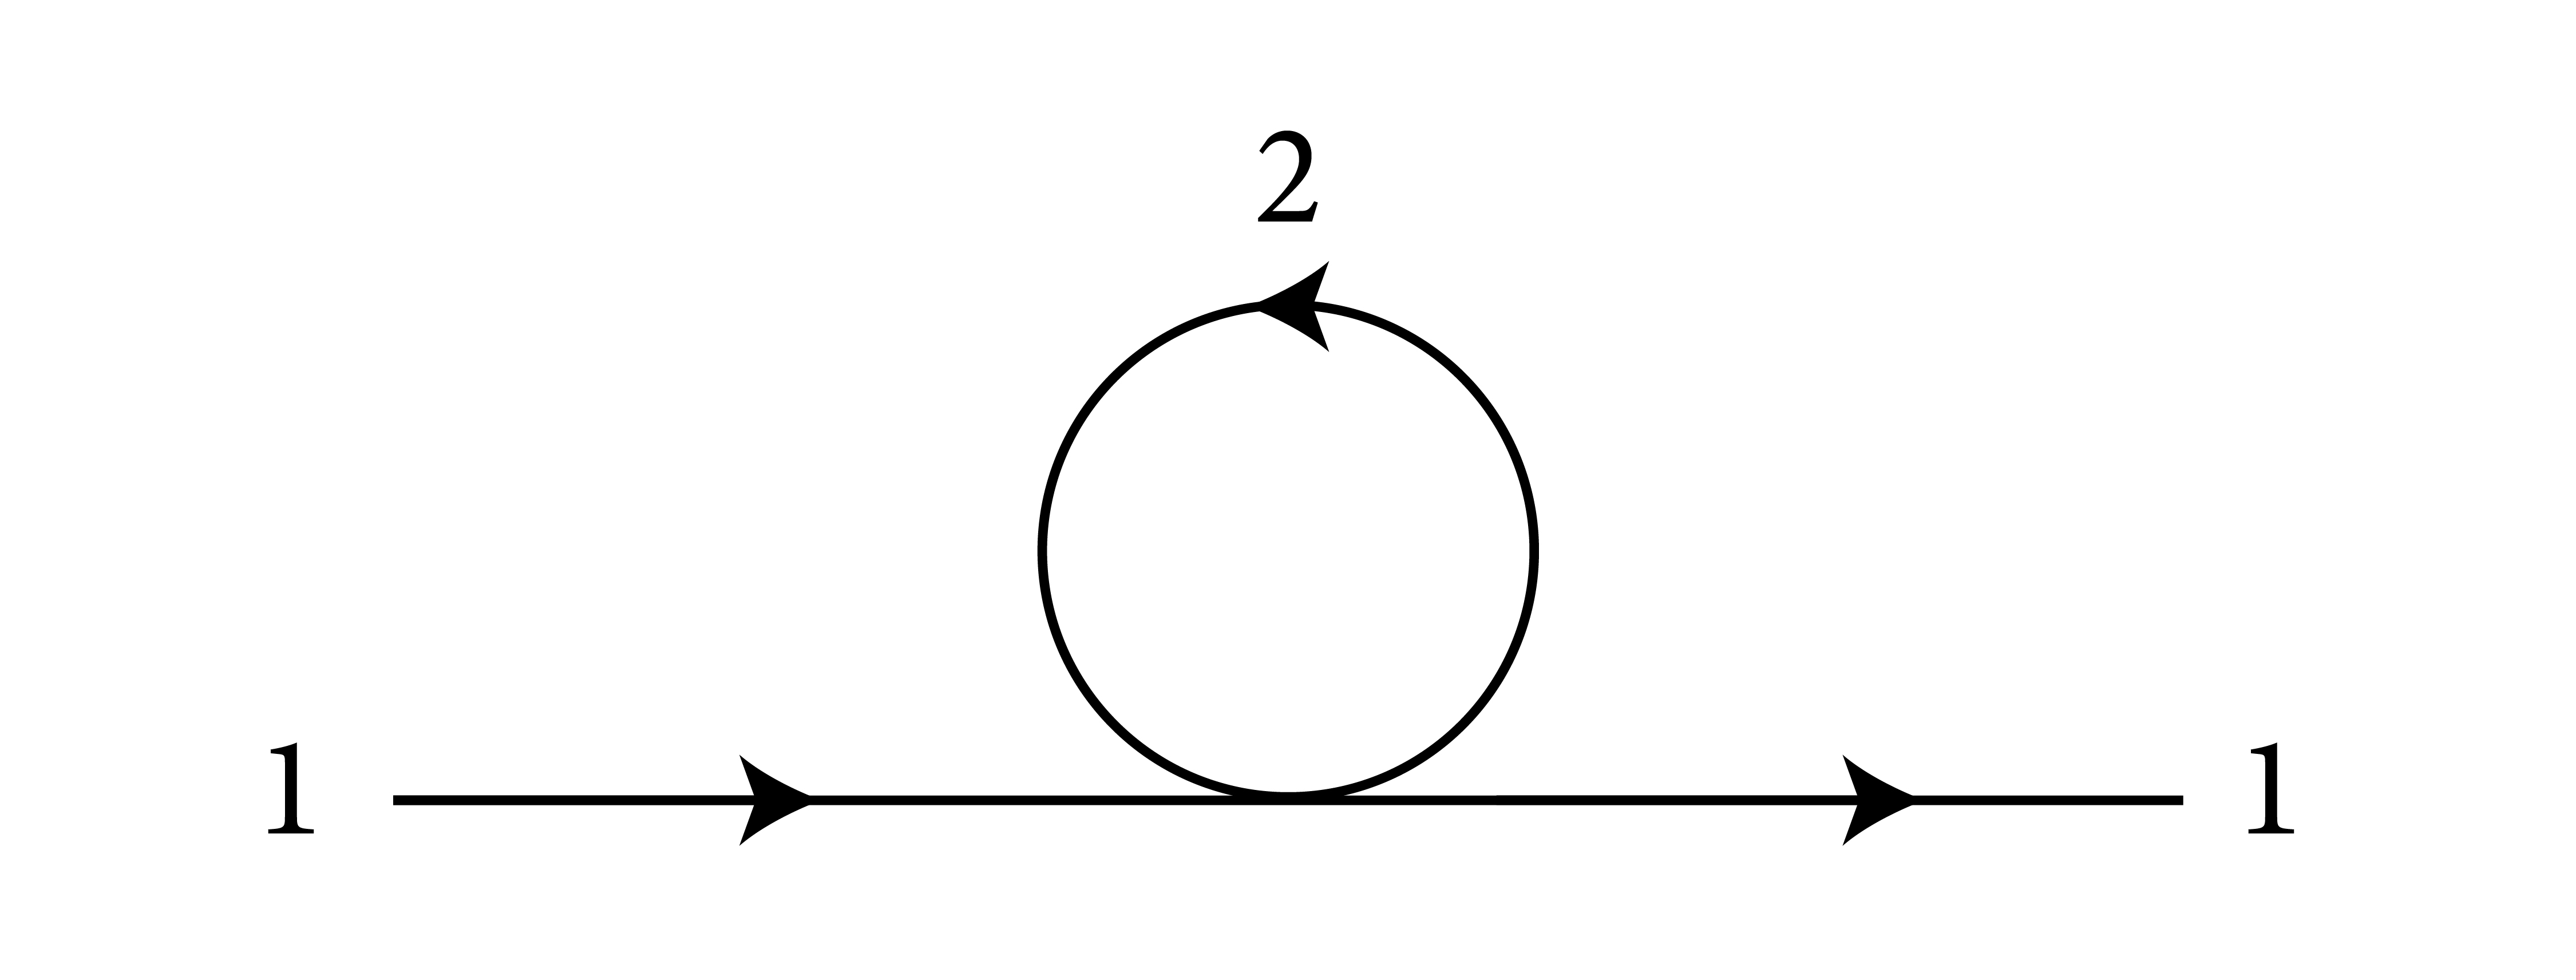
\includegraphics[width=0.6\textwidth]{images/2pointsoneloop.jpg}
    \caption{One loop correction to the two points function.}
    \label{fig:oneloop2}
\end{figure}
We are considering two correlators evaluated at the same points in $k$-space, since our objective is the term present in the r.h.s. of \eqref{kineticprototype}. 
In this case there always will be a delta arising from the diagrams whose argument is zero. This delta is the result of momentum conservation.
For this reason we will be dealing with a $\D_k$ defined as in \eqref{prop} instead of the full propagator\footnote{In equation \eqref{prop} we defined it 
with a zero superscript to indicate it was for the free theory, for the full propagator the definition would be $\tilde{G}_{k1}(\omga)=\delta(k-k_1)\D_k$},
ignoring the infinity arising from the aforementioned delta. \\
Using the Feynman rules explained in the last section, the form of the one loop correction to the two points function is
\begin{equation}
    \D_1^{1} = -4\frac{i}{2} \D^0_1\D^0_1 \sum_{2} \int \frac{d\omgatt_2}{2\pi} \Tint_{1221}\D^0_2\left[\frac{1}{\F_1}\left( \frac{1}{\G_1^*} - \frac{1}{\G_1}\right) +
    \frac{1}{\F_2}\left( \frac{1}{\G_2^*} - \frac{1}{\G_2}\right) 
    \right],
\end{equation}
\hl{THERE IS STILL A MISSING 2PI}\\
where the factor of four is the result of two possible ways of choosing the "incoming" particle and two possible ways of choosing the "outgoing" one.
%where the factor of two in front of the expression is the result of a factor of four, introduced to account for all possible ways to attach the external lines to the vertex 
%and obtain the same diagram, devided by the factor two present in the Feynman rules for the quartic vertex.\\ 
By expliciting the definition of $\G_i$ it is easy to see that
\begin{equation}
    \frac{1}{\F_i}\left( \frac{1}{\G_i^*} - \frac{1}{\G_i}\right) = \frac{2 i(\omgatt_i - \omga_i)}{\F_i}.
\end{equation}
The part of the integral where $i=2$ is antisymmetric for the exchange $\omgatt_2 - \omga_2 \rightarrow \omga_2 - \omgatt_2$, and is consequently null. Integrating
by again exploiting Jordan's lemma and the residue theorem the integral yealds
\begin{equation}
    \D_1^1 = 4\sum_2 \left( \D_1^0 \right)^2\frac{\omgatt_1 - \omga_1}{\F_1}n_2\Tint_{1212},
\end{equation}
where we used the definition of $n_k$ given in \eqref{freenwav}. It is important to remember that in our notation the subscripts indicate functional dependance whereas 
the superscripts indicate the perturbation order. \\
What we just obtained is an important result, by defining 
\begin{equation}
    \delta \omga_1 = 2\sum_2 n_2 \Tint_{1212} 
    \label{shiftilritorno}
\end{equation} 
we write the contributions up to one loop as
\begin{equation}
    \D_k^{\text{tot}} = \D_k^0 + 2\left( \D_k^0 \right)^2 \frac{\omgatt - \omga_k}{\F_k}\delta \omga_k. 
\end{equation}
This same result can be obtained by a shift $\omga_k \rightarrow \omga_k + \delta \omga_k$ in the Lagrangian, 
as substituting it into the free propagator and expanding for small $\delta \omga_k$ gives
\begin{align}
    \D_k^0(\omga_k + \delta\omga_k) &= \D_k^0(\omga_k) + \delta\omga_k\frac{\partial\D_k^0(\omga_k + \delta\omga_k)}{\partial \delta\omga_k}\big\rvert_{\delta\omga_k = 0} \\ 
    &=   \D_k^0(\omga_k) + 2\left( \D_k^0(\omga_k) \right)^2 \frac{\omgatt - \omga_k}{\F_k}\delta \omga_k.
\end{align} 
This is exactly the same shift to the frequency \eqref{shift_eq} we obtained in chapter 1 to avoid secolar growths in perturbation theory.
Recovering it through the QFT approach is a good sign of consistency. In this context it is usually called frequency renormalization. From now on we will indicate
as $\D_i$ the propagator with the shifted frequency.\\  
To find some nontrivial dynamics for the two point function we would need to go to higher loop orders, instead we will find the less cumbersome way of using 
\eqref{kineticprototype}. Thanks to this instead of evaluating two loop diagrams for the two point function, we have instead to evaluate one loop diagrams for the 
four points one. The next section is devoted to this task.\\  
\subsection{4-points functions}

Let us start with the lowest order contribution to the four point function. The only possible diagram is the one in figure \ref{fig:treefourpoints}.
\begin{figure}[ht]
    \centering
    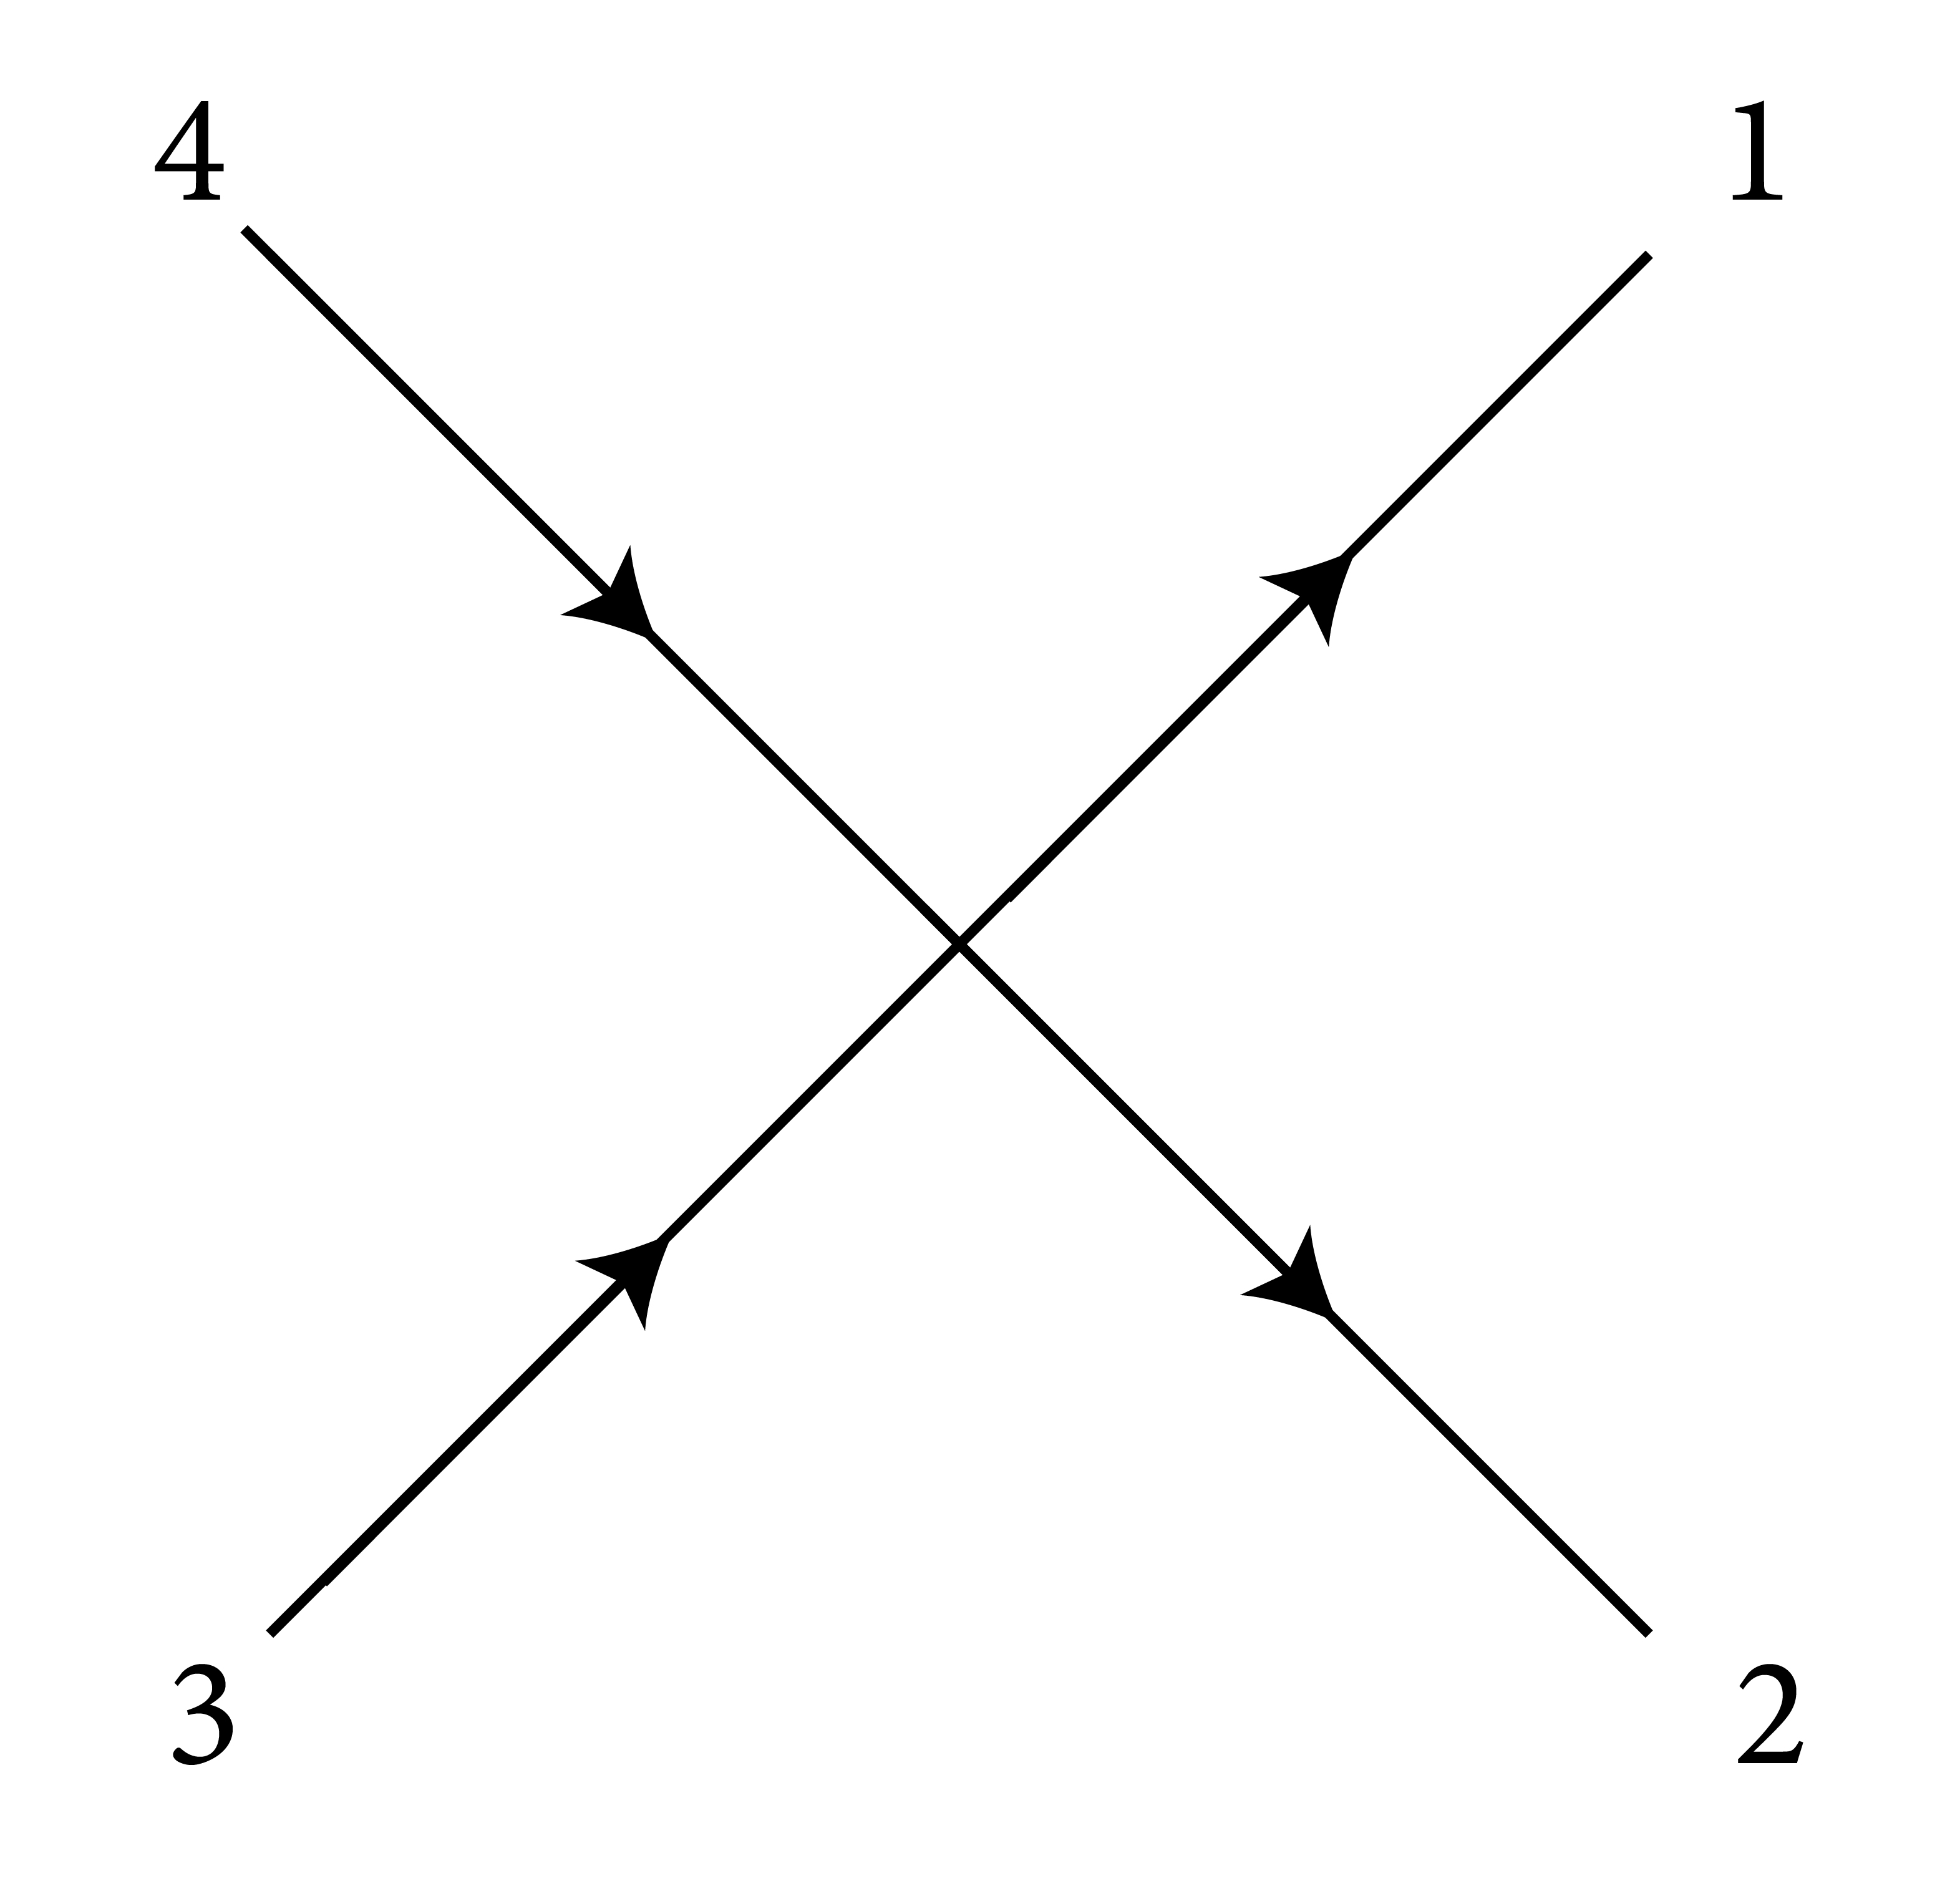
\includegraphics[width=0.4\textwidth]{images/quarticvertex.jpg}
    \caption{Lowest order diagram for the four points function.}
    \label{fig:treefourpoints}
\end{figure}
The corresponding expression is
\begin{equation}
    \langle \aonet \atwot \athreestart\afourstart \rangle_{0} = -4\frac{i}{2} \Tint_{1234}\left(\dfrac{1}{\G_1^*\F_1^{}}+\dfrac{1}{\G_2^*\F_2^{}}-\dfrac{1}{\G_3^{}\F_3^{}}
    -\dfrac{1}{\G_4^{}\F_4^{}}\right)\D_1^0\D_2^0\D_3^0\D_4^0 2\pi \delta(\delomegatt^{12}_{34})\delta^{12}_{34},
    \label{4pointfreq}
\end{equation}
where $\tilde{a}_i^{}$ is the Fourier transform of $a_i^{}(t_i)$ and the factor of four comes again from the different ways of attaching "incoming" and "outcoming" 
propagators to the vertex.\\
As we are interested in the time domain let us antitransform the four point function, already fixing $t_1 = t_2 = t_3 = t_4 = t$. The objective is
\begin{equation}
    \langle\aone(t) \atwo(t) \athreestar(t) \afourstar(t) \rangle_0 = \int \frac{d\omgatt_1}{2\pi}\frac{d\omgatt_2}{2\pi}\frac{d\omgatt_2}{2\pi}\frac{d\omgatt_2}{2\pi}
    e^{i(\omgatt_1 + \omgatt_2  -\omgatt_3 - \omgatt_4)t} \langle \aonet \atwot \athreestart\afourstart \rangle_{0}.
\end{equation}
We substitute \eqref{4pointfreq} into it and use the delta function over frequencies to solve one of the three integrals. Then the remaning three integrals may 
be performed by properly closing the integration path and using the residue theorem. The result, again using \eqref{freenwav}, is
\begin{equation}
    \langle\aone(t) \atwo(t) \athreestar(t) \afourstar(t) \rangle_0 = 2\Tint_{1234}n_1 n_2 n_3 n_4\left( \frac{1}{n_1}+\frac{1}{n_2}-\frac{1}{n_3}-\frac{1}{n_4} \right)
    \frac{1}{\delomega^{34}_{12} + i\gamma_{1234}},
\end{equation}  
where $\gamma_{1234} = \gamma_1 + \gamma_2 + \gamma_3 + \gamma_4$. \\

There are four  one loop diagrams contributing to the four point function. Three of them, in figure \ref{fig:quarticoneloop}, are composed from two quartic vertices.
The remaining one is built from one sextic vertex.
\begin{figure}[ht]
    \centering
    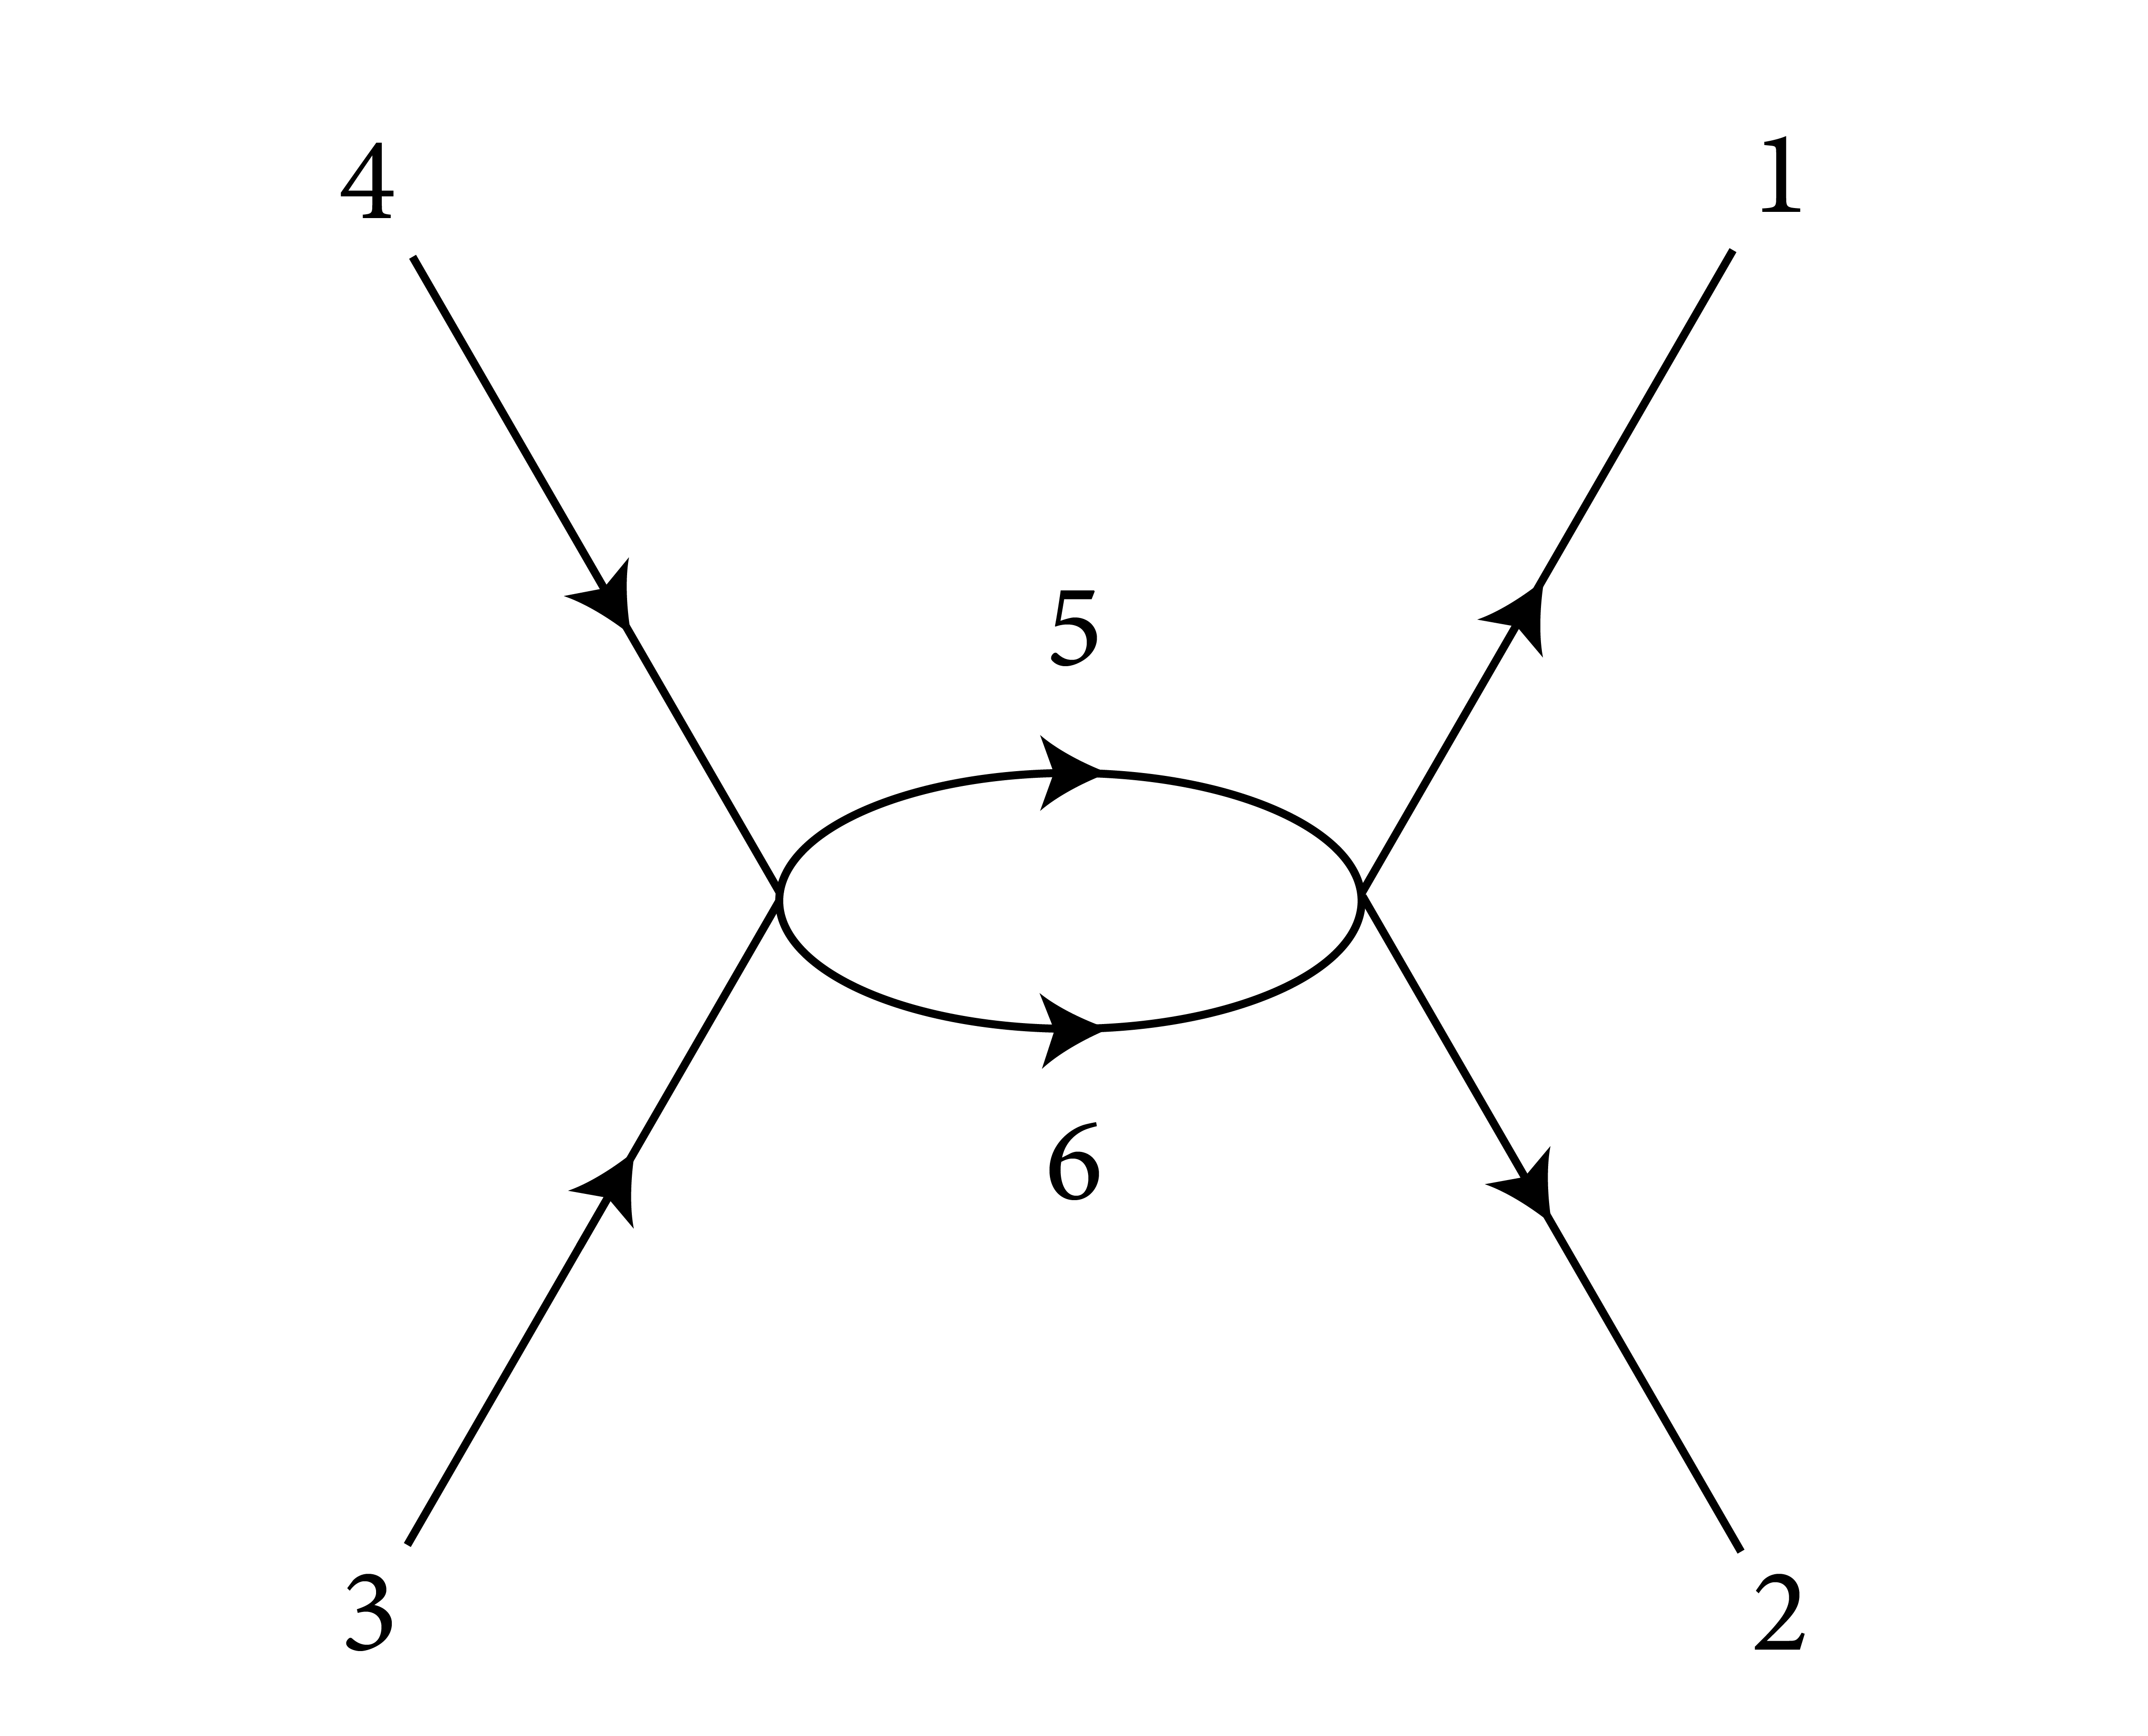
\includegraphics[width=0.4\textwidth]{images/schanneloneloop.jpg}\\
    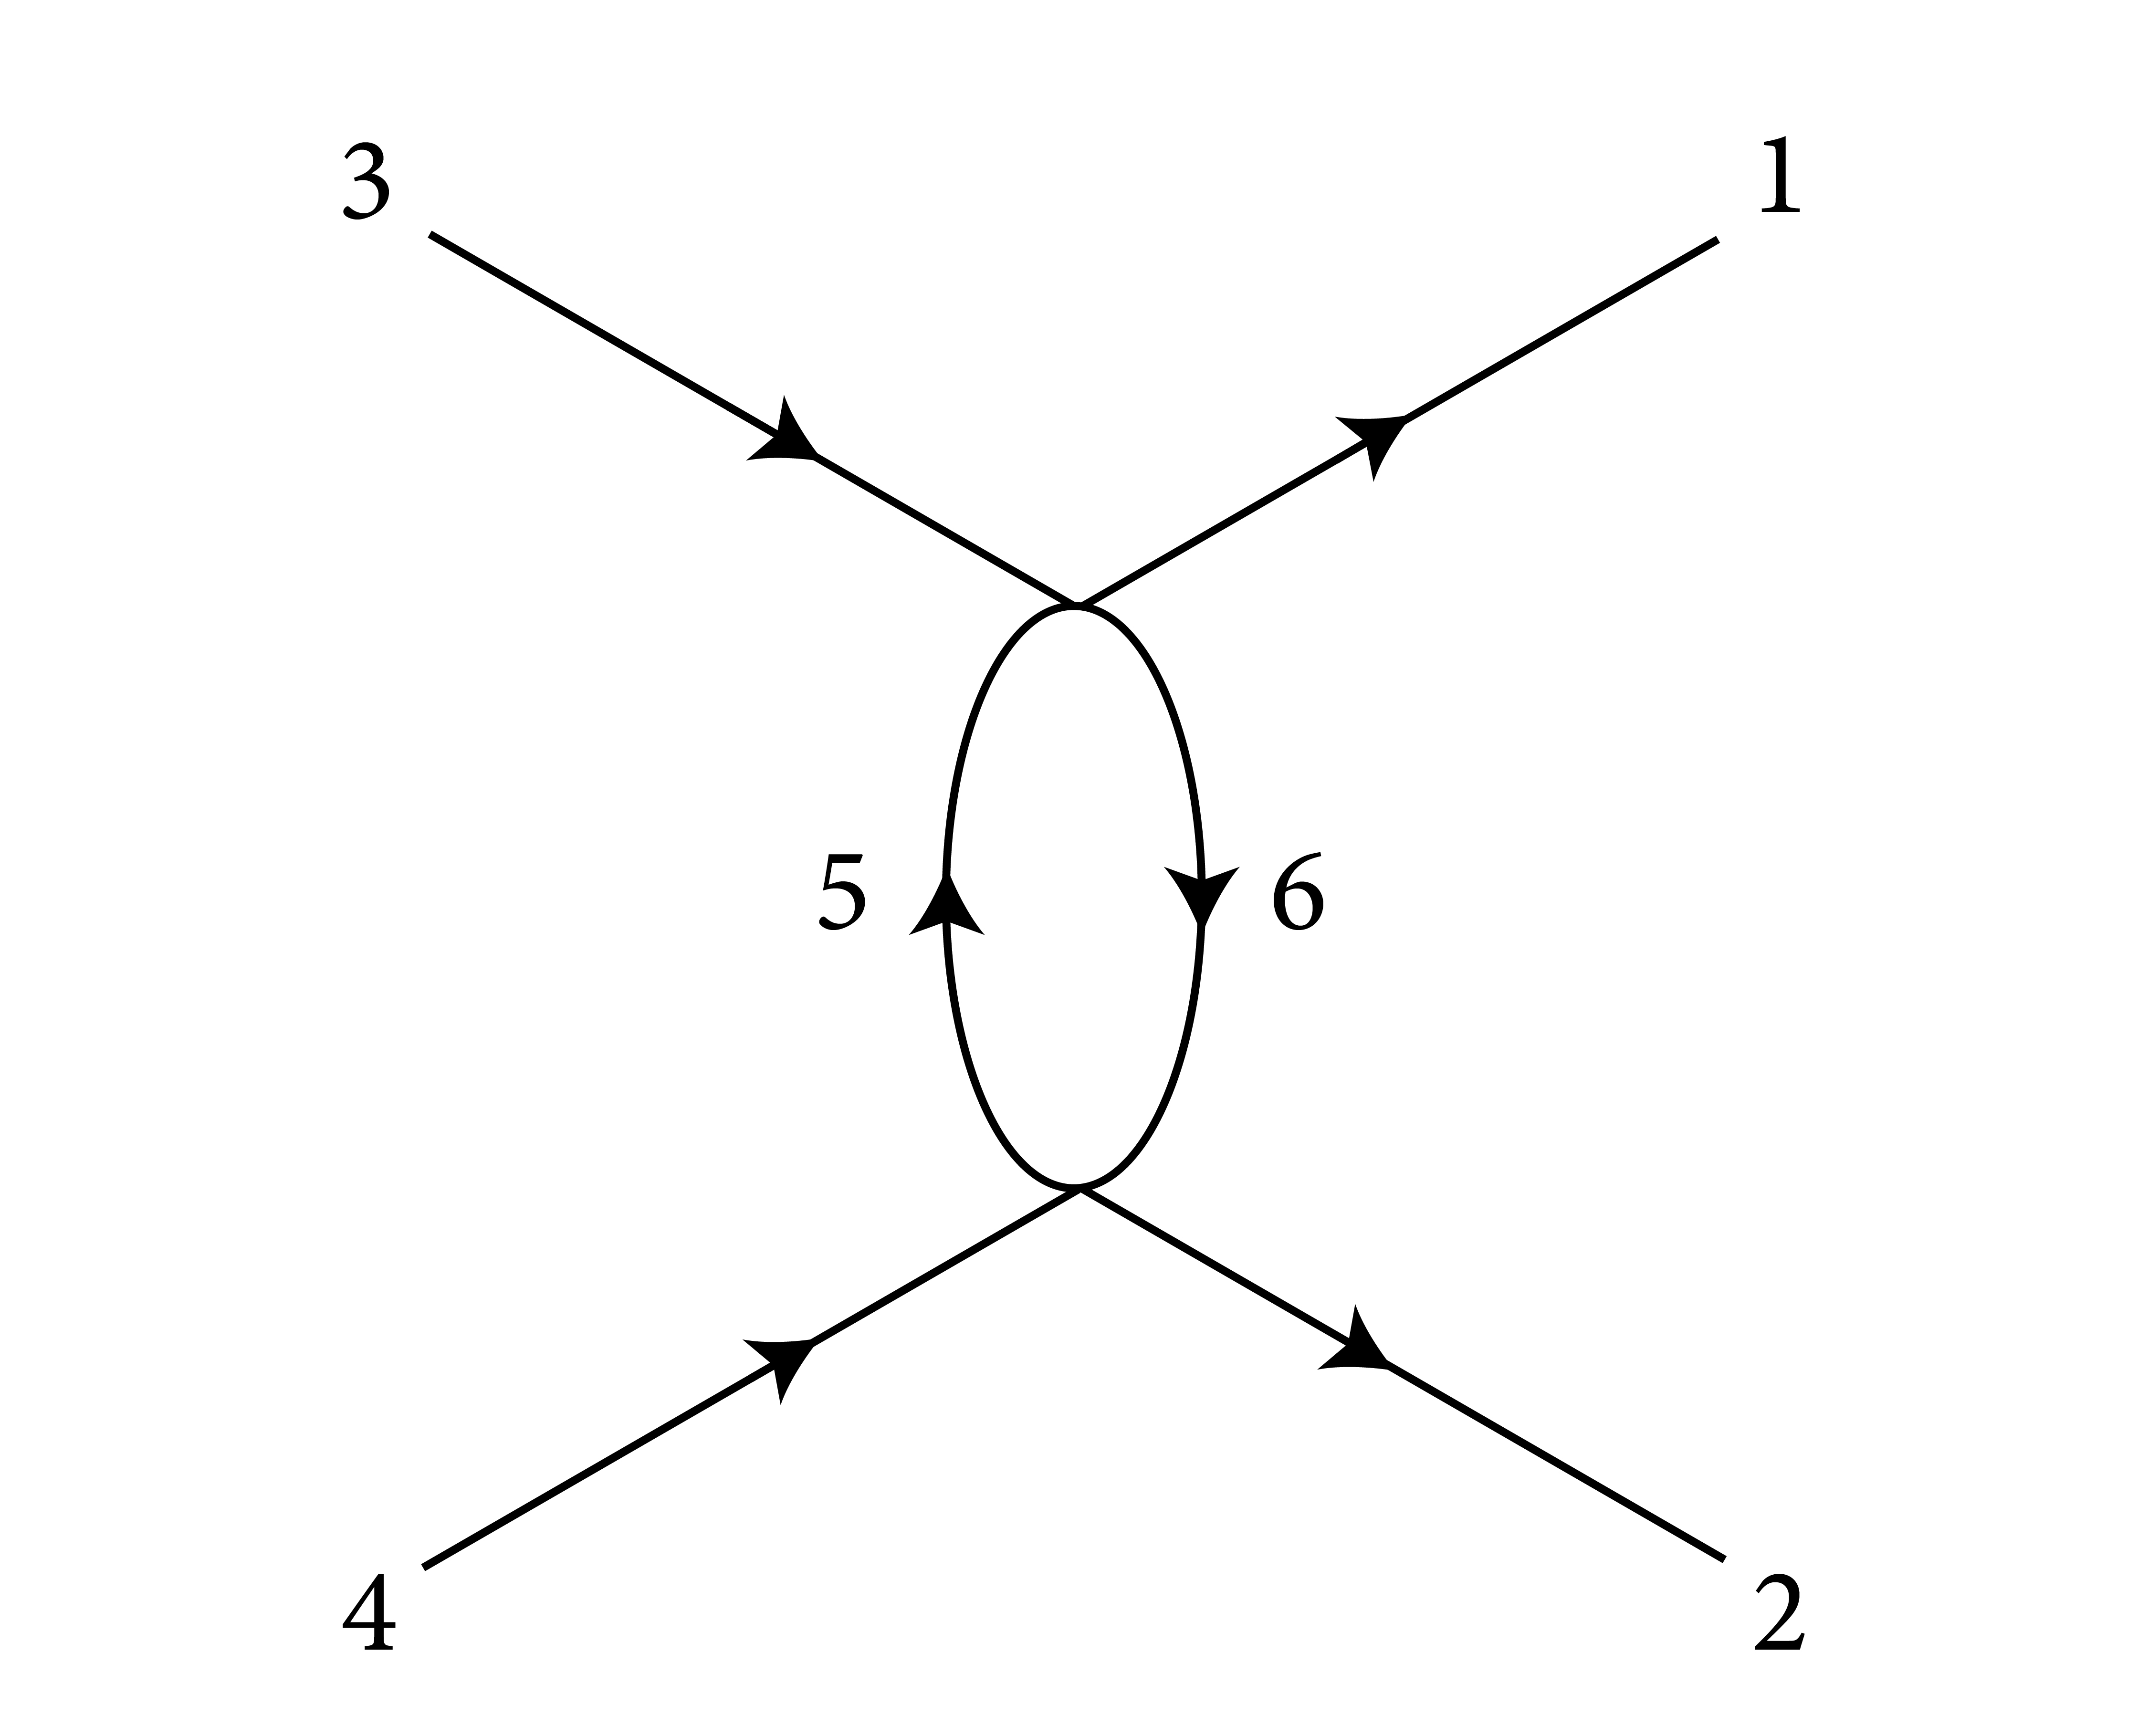
\includegraphics[width=0.4\textwidth]{images/tchanneloneloop.jpg}
    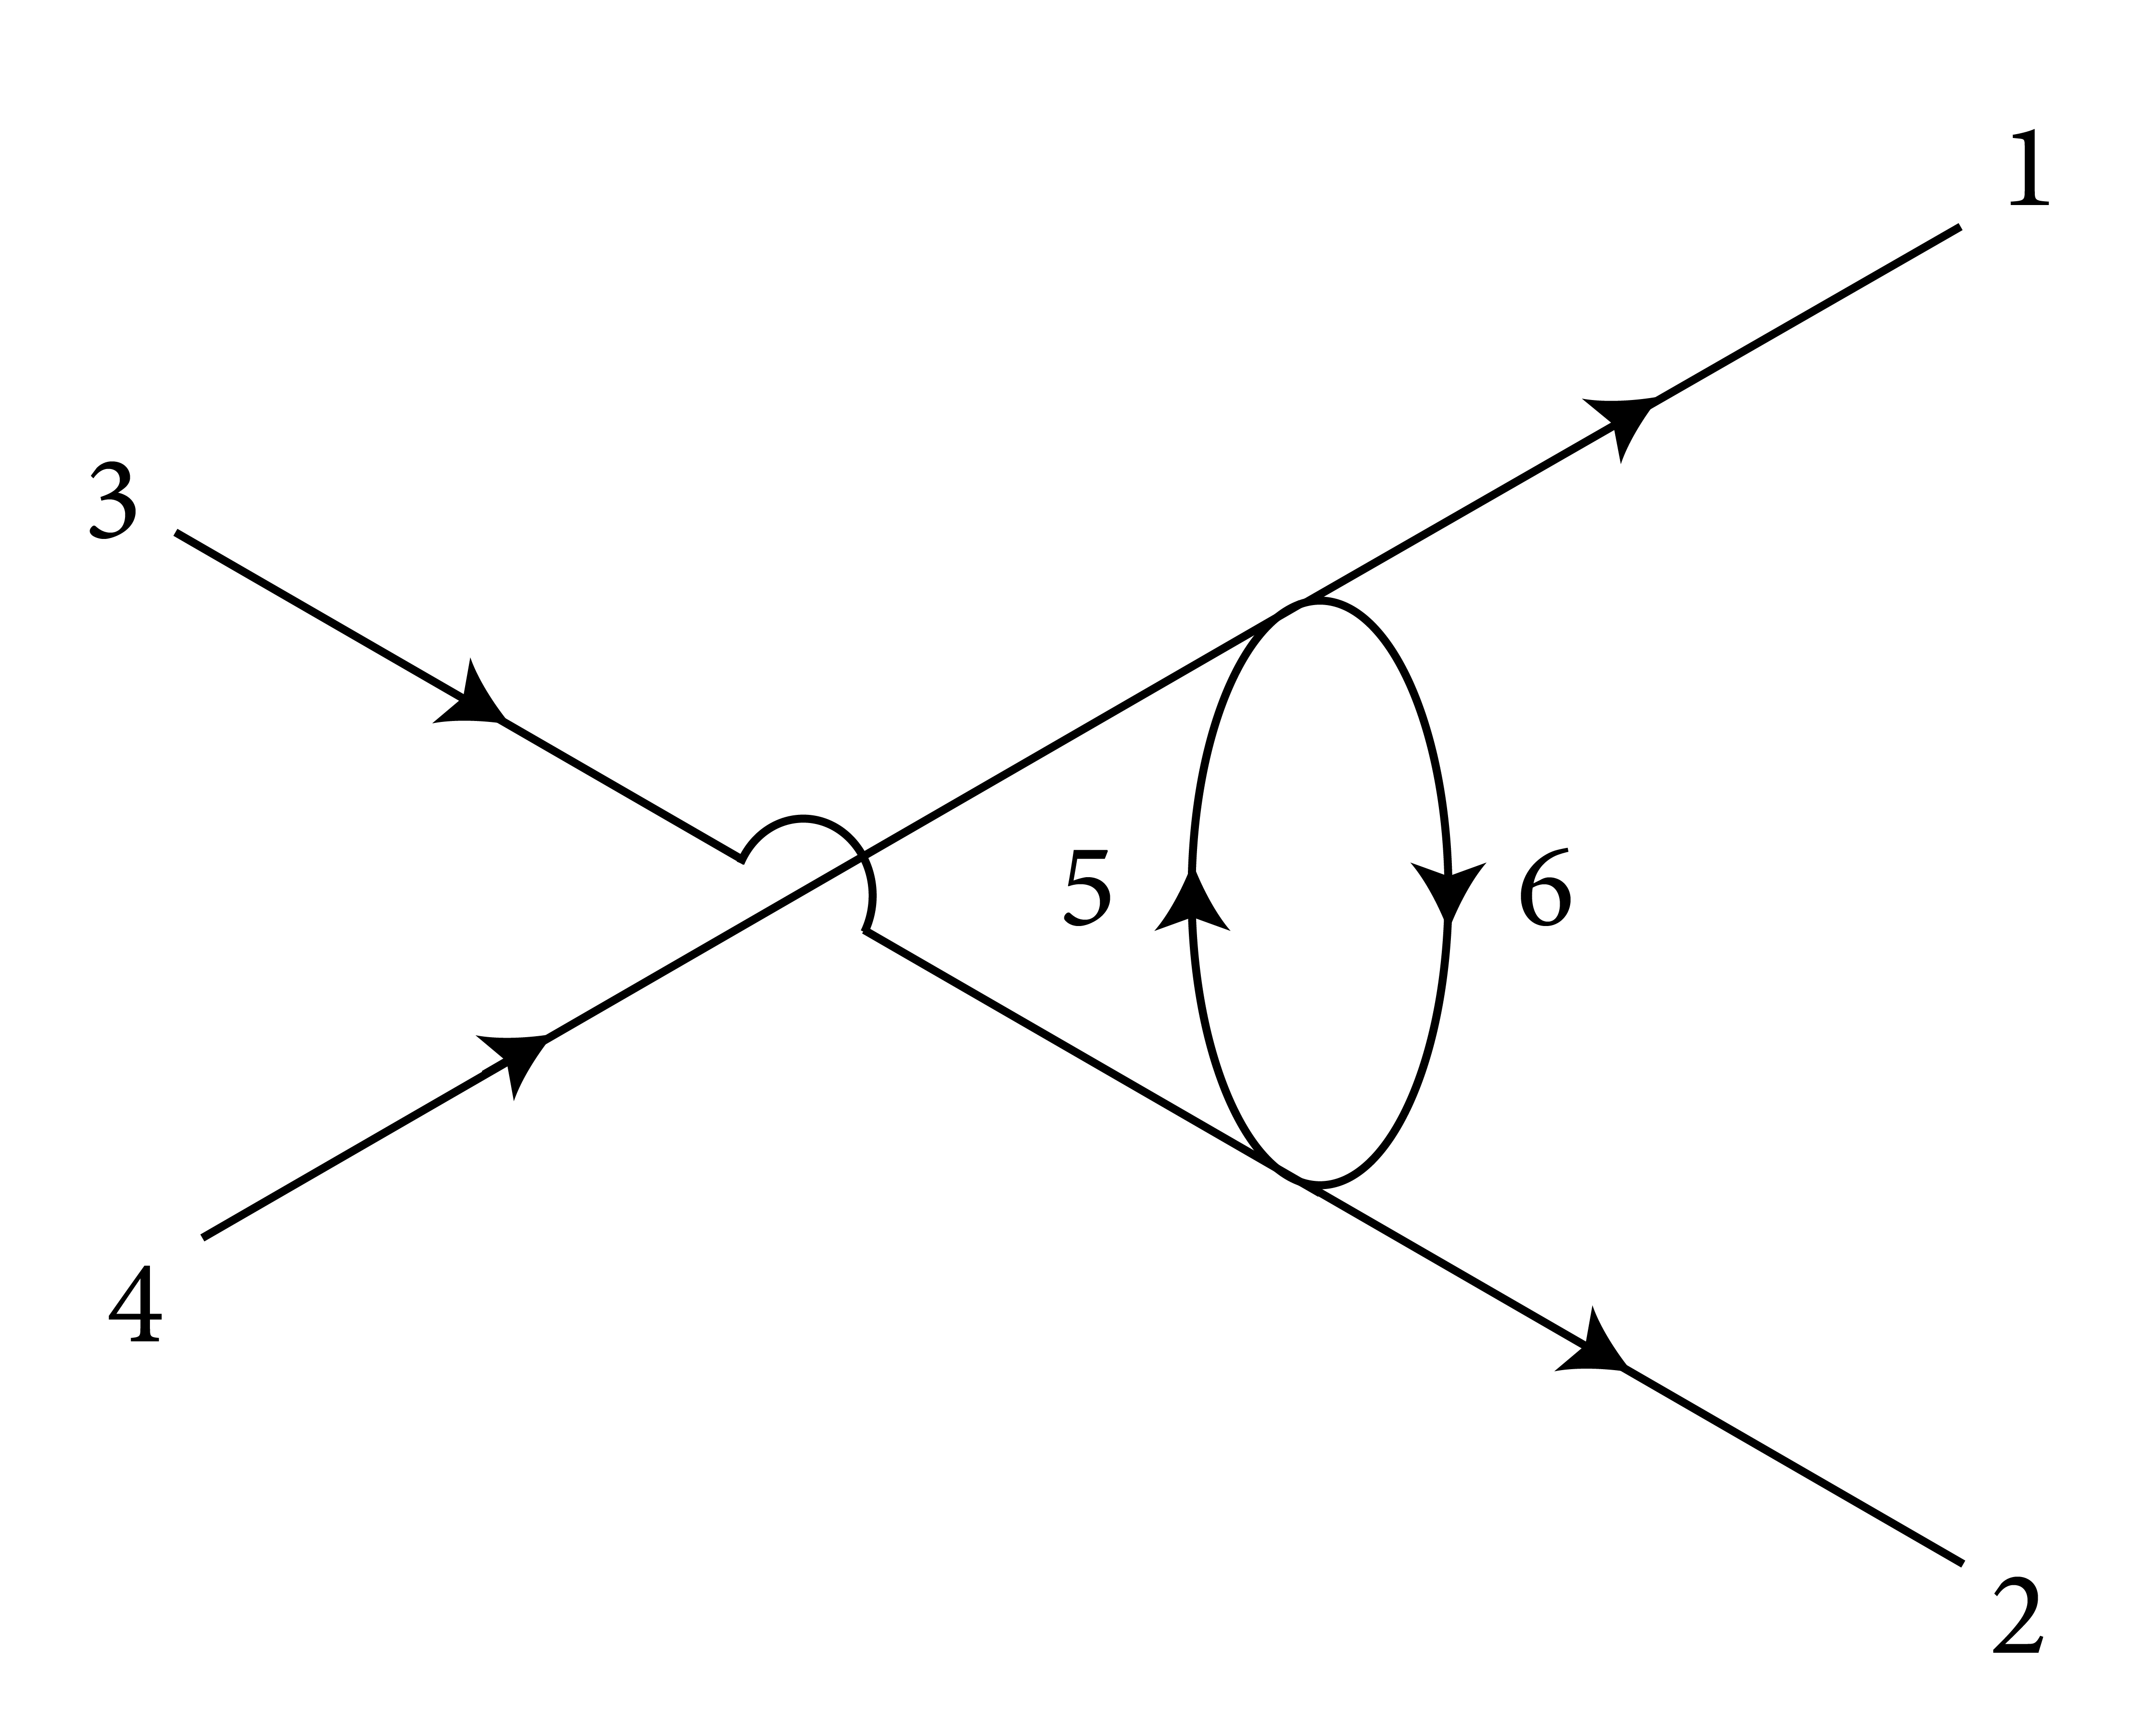
\includegraphics[width=0.4\textwidth]{images/uchanneloneloop.jpg}
    \caption{Quartic one loop diagrams.}
    \label{fig:quarticoneloop}
\end{figure} 
Let us start from the first diagram in figure \ref{fig:quarticoneloop}, it contains four external lines, two internal ones and two vertices. Its corresponding expression is
\begin{multline}
    -8\pi^2\sum_{56}\int \frac{d\omgatt_5}{2\pi}\frac{d\omgatt_6}{2\pi}\delta(\delomegatt^{34}_{56})\delta(\delomegatt^{56}_{12})\Tint_{5634}\Tint_{1256}\delta^{56}_{34}
    \delta^{12}_{56}\D_1^0\D_2^0\D_3^0\D_4^0\D_5^0\D_6^0 \\ 
    \times \left(\dfrac{1}{\G_5^*\F_5^{}}+\dfrac{1}{\G_6^*\F_6^{}}-\dfrac{1}{\G_3^{}\F_3^{}}
    -\dfrac{1}{\G_4^{}\F_4^{}}\right)\left(\dfrac{1}{\G_1^*\F_1^{}}+\dfrac{1}{\G_2^*\F_2^{}}-\dfrac{1}{\G_5^{}\F_5^{}}
    -\dfrac{1}{\G_6^{}\F_6^{}}\right).
    \label{schannel}
\end{multline}
Here the symmetry factor is given by the 16 possible ways of attaching the lines to the vertices and still results in an equivalent diagram. 
An additional factor of $\dfrac{1}{2}$ has to be included, coming from perturbation theory. The origin of this latter term is again out of the scope of this thesis, the reader is directed
to any QFT textbook to better understand it. INtuitively it corresponds to the $\dfrac{1}{2}$ term appearing in the second order of a Taylor expansion. \\
We may readily resolve one of the integrals by using a delta function, so that now $\omgatt_6 = \omgatt_3 + \omgatt_4 - \omgatt_5$. The second delta will now not depend 
anymore on the integration variable $\omgatt_5$, only enforcing conservation of energy. \\
The integrand is made of 16 terms summed, before integrating them explicitely we shall prepare some identities. We will need all possible combinations of 
the terms in \eqref{schannel} depending on $\omgatt_5$, remembering that, thanks to the delta function, $\G_6$ and $\D_6$ depends on it as well\footnote{
    Remember that $\frac{1}{\F_i \G_i}\D^{}_i = \G_i^*$, implying that $\G^{}_i$ or $\G^{*}_i$ will always appear in the numerator.
}. \\
All following identities can be easily obtained by substituting the definitions of $\D$ and $\G$, and subsequently closing the integration path either 
on the upper half plane (UHP) or the lower one (LHP). They are
\begin{align}
    &\int \frac{d\omgatt_5}{2\pi} \D_5 \D_6 \underset{LHP}{=} \frac{2n_5n_6\gamma_{56}}{\left( \omgatt_3 + \omgatt_4 - \omga_5 - \omga_6\right)^2 + \gamma^2_{56}}, 
    \label{identity1}\\
    &\int \frac{d\omgatt_5}{2\pi} \G_5 \D_6 \underset{UHP}{=} \frac{in_6}{\omgatt_3 + \omgatt_4 - \omga_5 - \omga_6 +i\gamma_{56}}, \\
    &\int \frac{d\omgatt_5}{2\pi} \G_6 \D_5 \underset{LHP}{=} \frac{in_5}{\omgatt_3 + \omgatt_4 - \omga_5 - \omga_6 +i\gamma_{56}}, \\
    &\int \frac{d\omgatt_5}{2\pi} \G_5^{} \G_6^* \underset{UHP}{=} 0, \\
    &\int \frac{d\omgatt_5}{2\pi} \D_5 \underset{LHP}{=} n_5, \label{identity5}\\
    &\int \frac{d\omgatt_5}{2\pi} \G_5\G_6 \underset{LHP}{=} \frac{-i}{\omgatt_3 + \omgatt_4 - \omga_5 - \omga_6 +i\gamma_{56}}.
    \label{identity6}
\end{align}  
Now let us move to the full integral. There is a common factor of
\begin{equation*}
    -4\pi\delta(\delomegatt^{34}_{12})\sum_{56}\Tint_{5634}\Tint_{1256}\D_1^0\D_2^0\D_3^0\D_4^0
\end{equation*}
in front of the integral. Then there is the $d\omgatt_5$ integration of 16 terms. Integrating them, using identities \eqref{identity1}-\eqref{identity6},
is a tedious but straightforward process. \hl{FORSE AGGIUNGI IN APPENDICE CONTI} The complete result is 
\begin{multline}
    -4\pi\delta(\delomegatt^{34}_{12})\sum_{56}\Tint_{5634}\Tint_{1256}\D_1^0\D_2^0\D_3^0\D_4^0 \left\{ -\frac{n_6}{\F_5}-\frac{n_5}{\F_6}\right. + 
    \frac{1}{\left( \omgatt_3 + \omgatt_4 - \omga_5 - \omga_6\right)^2 + \gamma^2_{56}}\\
    \times \left[
    i(n_5 + n_6)\left(\dfrac{1}{\G_1^*\F_1^{}}+\dfrac{1}{\G_2^*\F_2^{}}-\dfrac{1}{\G_3^{}\F_3^{}}
    -\dfrac{1}{\G_4^{}\F_4^{}}\right)\left( \omgatt_3 + \omgatt_4 - \omga_5 - \omga_6\right) + 
    \right.\\
    \left.\left.
    \gamma_{56}\left((n_5 + n_6)\left(\dfrac{1}{\G_1^*\F_1^{}}+\dfrac{1}{\G_2^*\F_2^{}}+\dfrac{1}{\G_3^{}\F_3^{}}
    +\dfrac{1}{\G_4^{}\F_4^{}}\right) - 2n_5n_6 \left(\dfrac{1}{\G_1^*\F_1^{}}+\dfrac{1}{\G_2^*\F_2^{}}\right)\left(\dfrac{1}{\G_3^{}\F_3^{}}
    +\dfrac{1}{\G_4^{}\F_4^{}}\right)\right)
    \right]\right\}.
    \label{schannelfullcontribution}
\end{multline}
The second diagram in figure \ref{fig:quarticoneloop} contains the same elements, but with permuted indexes. Its mathematical form is 
\begin{multline}
    -16\pi^2\sum_{56}\int \frac{d\omgatt_5}{2\pi}\frac{d\omgatt_6}{2\pi}\delta(\delomegatt^{46}_{52})\delta(\delomegatt^{35}_{16})\Tint_{2546}\Tint_{3516}\delta^{25}_{46}
    \delta^{35}_{16}\D_1^0\D_2^0\D_3^0\D_4^0\D_5^0\D_6^0 \\ 
    \times \left(\dfrac{1}{\G_5^*\F_5^{}}+\dfrac{1}{\G_2^*\F_2^{}}-\dfrac{1}{\G_6^{}\F_6^{}}
    -\dfrac{1}{\G_4^{}\F_4^{}}\right)\left(\dfrac{1}{\G_1^*\F_1^{}}+\dfrac{1}{\G_6^*\F_6^{}}-\dfrac{1}{\G_5^{}\F_5^{}}
    -\dfrac{1}{\G_3^{}\F_3^{}}\right).
    \label{tchannel}
\end{multline}
The ways to compose the diagram are 32, resulting in a symmetry factor of 16. Integrating through 
identities similar to \eqref{identity1}-\eqref{identity6}, the expression becomes
\begin{multline}
    -8\pi\delta(\delomegatt^{34}_{12})\sum_{56}\Tint_{2546}\Tint_{6135}\D_1^0\D_2^0\D_3^0\D_4^0 \left\{ -\frac{n_6}{\F_5}-\frac{n_5}{\F_6}\right. +
    \frac{1}{\left( \omgatt_1 + \omga_6 - \omgatt_3 - \omga_5\right)^2 + \gamma^2_{56}}\\
    \times \left(
    i(n_6-n_5)\left(\dfrac{1}{\G_1^*\F_1^{}}+\dfrac{1}{\G_2^*\F_2^{}}-\dfrac{1}{\G_3^{}\F_3^{}}
    -\dfrac{1}{\G_4^{}\F_4^{}}\right)\left(\omgatt_1 + \omga_6 - \omgatt_3 - \omga_5\right) + 
    \right.\\
    \left.\left.
    \gamma_{56}\left[(n_6-n_5 )\left(\dfrac{1}{\G_1^*\F_1^{}}-\dfrac{1}{\G_2^*\F_2^{}}-\dfrac{1}{\G_3^{}\F_3^{}}
    +\dfrac{1}{\G_4^{}\F_4^{}}\right) + 2n_5n_6 \left(\dfrac{1}{\G_2^*\F_2^{}}-\dfrac{1}{\G_4^{}\F_4^{}}\right)\left(\dfrac{1}{\G_1^*\F_1^{}}-\dfrac{1}{\G_3^{}\F_3^{}}
    \right)\right)
    \right]\right\}.
    \label{tchannelfullcontribution}
\end{multline}    
The third diagram is equal to the second one, just with the two outgoing lines swapped. Consequently its contribution can be obtained from 
\eqref{tchannelfullcontribution} by the permutations $k_3 \leftrightarrow k_4$, $\omgatt_3 \leftrightarrow\omgatt_4$ and $\omga_3 \leftrightarrow\omga_4$.\\

The last contribution to be considered at order $\Tint^2$ is the one in figure \ref{fig:sexticoneloop}. It may be regarded at the equivalent of the diagram in figure 
\ref{fig:oneloop2}, but for four points functions. We may already suspect it to be related to frequency renormalization.\\

\begin{figure}[ht]
    \centering
    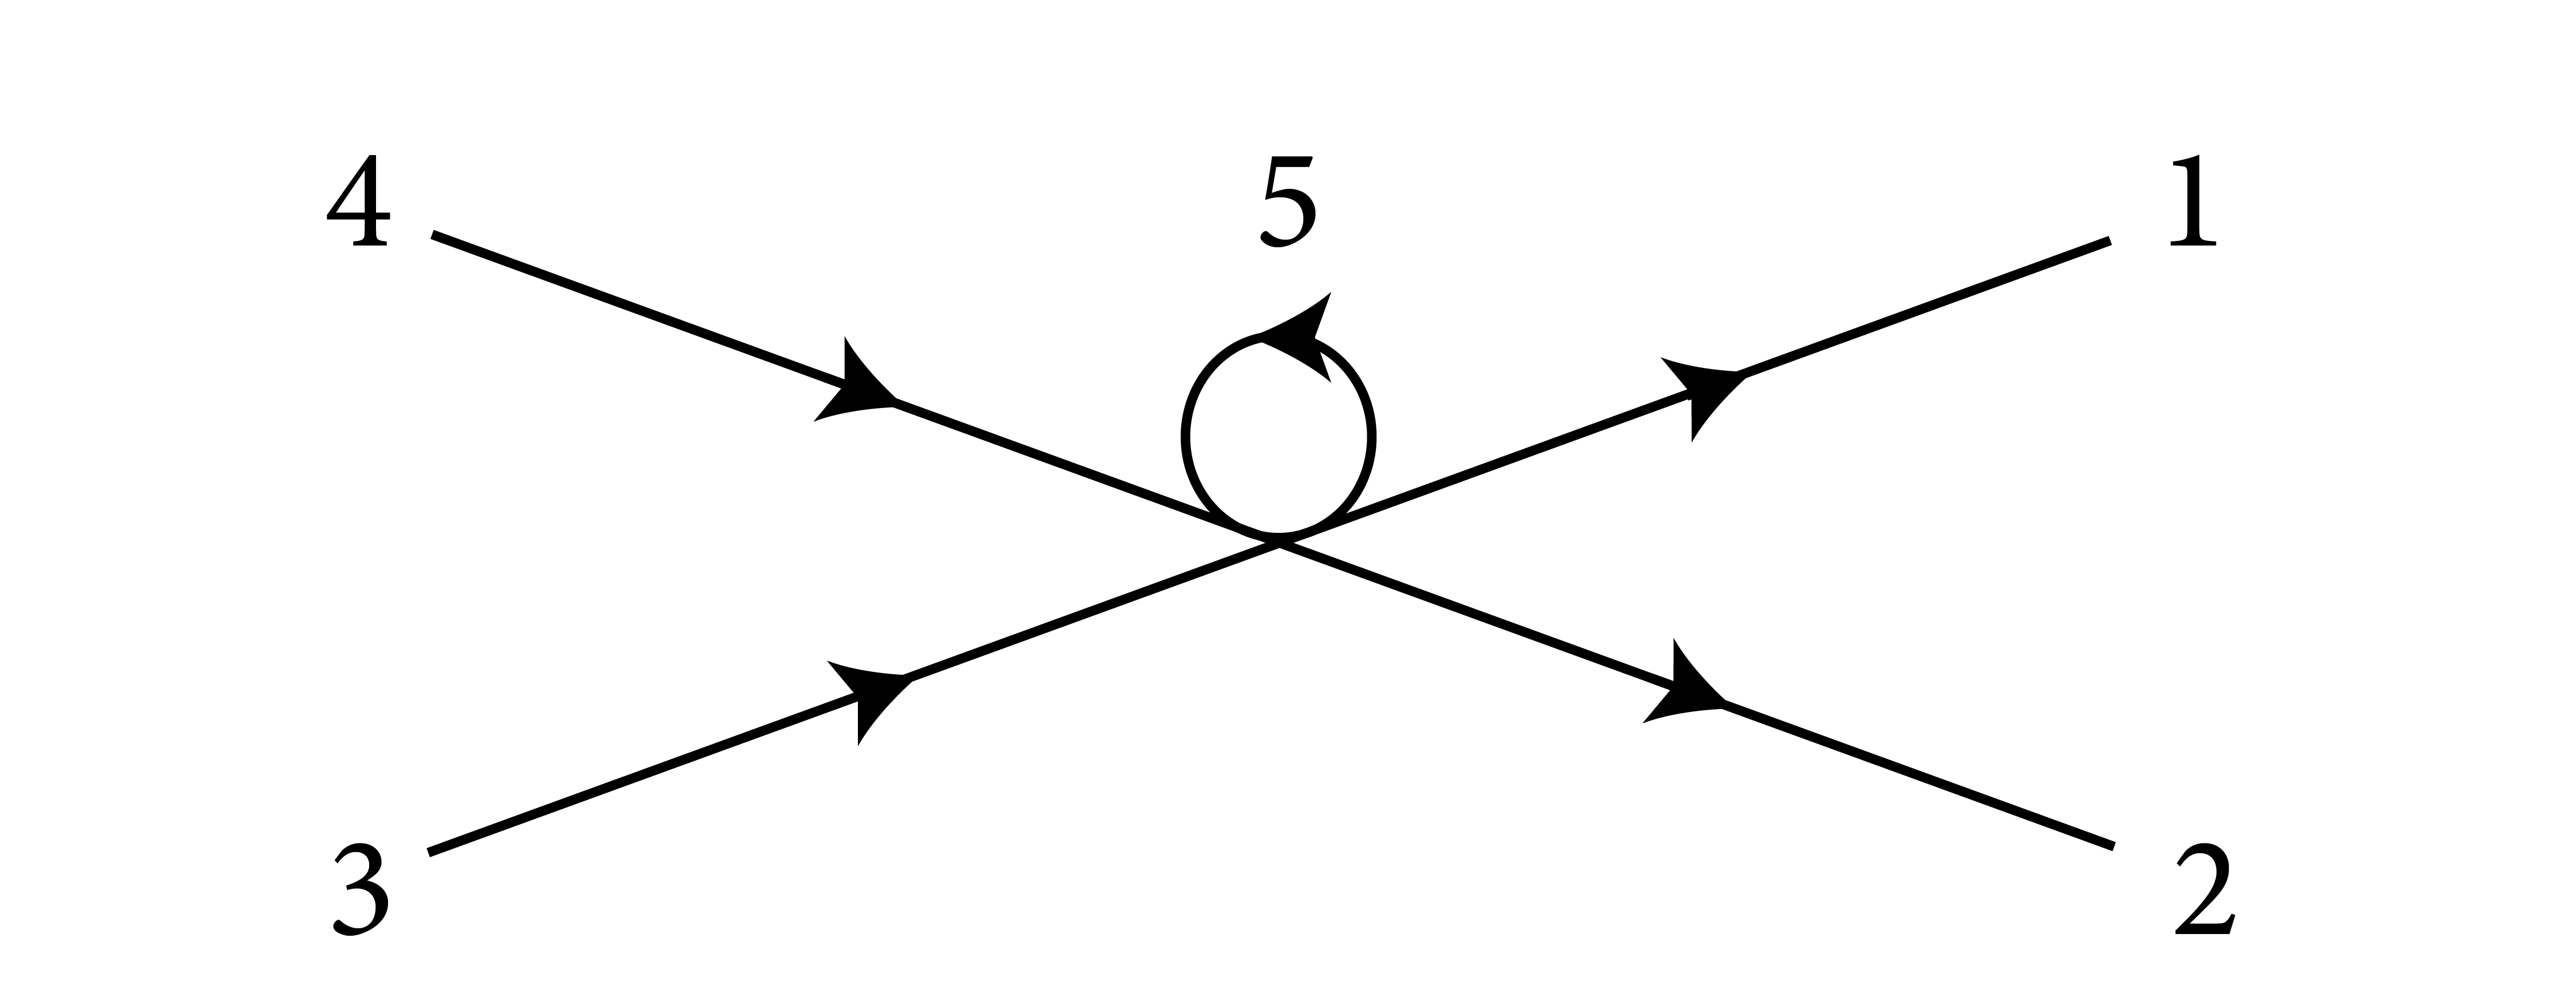
\includegraphics[width=0.5\textwidth]{images/sexticdiagram.jpg}
    \caption{Sextic one loop diagram.}
    \label{fig:sexticoneloop}
\end{figure}
We have again to consider all possible ways of attaching lines to vertices, there are \\$3!\cdot3! = 36$. However in this case different ways of building the diagram do not correspond to 
equal mathematical expressions. In the case of the first diagram in figure \ref{fig:quarticoneloop} the exchange of incoming lines would result in a term $\Tint_{2156}$
instead of $\Tint_{1256}$. Thanks to the symmetry properites of $\Tint$ the two contributions are equal and all possible permutations are accounted for in the symmetry factor.
This generalizes to quartic diagrams as the permutations always involve indexes under whose exchange the coupling $\Tint$ is symmetryc.\\ 
In the case of figure \ref{fig:sexticoneloop} it is not true that all permutations result in the same contribution, we have thus to parse through them all. The diagram 
is made of four external lines, one internal one and a sextic vertex. We exchange labels $4$ and $5$ in the sextic vertex feynman rules, as to have lines $3$ and 
$4$ both incoming as in figure \ref{fig:sexticoneloop}. The relative expression is thus  
\begin{equation}
    -2\pi \sum_{k5}\int\frac{d\omgatt_5}{2\pi} \frac{1}{\F_k}\left(\Tint_{123k}\Tint_{k545}\delta^{12}_{3k}
    \delta^{k5}_{45} + \text{permutations}\right)\delta(\delomegatt^{12}_{34})
    \D_1^0\D_2^0\D_3^0\D_4^0\D_5^0.
\end{equation}
We can resolve the integral over $\omgatt_5$, as the only term depending on it is $\D_5$, using identity \eqref{identity5}. The result is
\begin{equation}
    -2\pi \delta(\delomegatt^{12}_{34})\D_1^0\D_2^0\D_3^0\D_4^0 \sum_{k5}
    \frac{n_5}{\F_k}\left(\Tint_{123k}\Tint_{k545}\delta^{12}_{3k}
    \delta^{k5}_{45} + \text{permutations}\right).
\end{equation}
Writing all possible permutations of indexes $(1,2,5)$ and $(3,4,6)$ from $\Tint_{123k}\Tint_{k546}$, imposing $k_5 = k_6$ and using the symmetries of $\Tint$ 
reduces the unequivalent terms' number to seven. In four of them one of the deltas over wavenumbers may be used to eliminate the integration over $k$. After slightly manipulating
and renaming the dummy indexes, the full result is 
\begin{multline}
    -2\pi \delta(\delomegatt^{12}_{34})\D_1^0\D_2^0\D_3^0\D_4^0\left[ 4\sum_5\Tint_{1234}\delta^{12}_{34} \sum_{j=1}^{4}\frac{\Tint_{j5j5}}{\F_j}n_5 + \right.\\ 
    \left.  2\sum_{56}\left( \frac{n_5}{\F_6} + \frac{n_6}{\F_5} \right)\left( \Tint_{1256}\Tint_{5634}\delta^{12}_{56}\delta^{56}_{34} 
    + 2\Tint_{2546}\Tint_{6153}\delta^{25}_{46}\delta^{61}_{53}
    + 2\Tint_{5146}\Tint_{6253}\delta^{51}_{46}\delta^{62}_{53} \right) \right].
    \label{sexticfullcontribution}
\end{multline}
\\
We can rewrite the first part of \eqref{sexticfullcontribution}, using \eqref{shiftilritorno}, as 
\begin{equation}
    -4\pi \delta(\delomegatt^{12}_{34})\D_1^0\D_2^0\D_3^0\D_4^0\sum_{j=1}^{4}\frac{\delta \omga_i}{\F_i}.
    \label{shiftsextic}
\end{equation}
If we were to peform the frequency shift in $\Lag$, a new quartic interaction term would appear along with its Feynman's rule. 
This term would manifest itself, at this order of perturbation theory, in a diagram similar to the one in figure \ref{fig:treefourpoints}, 
yealding exactly the same contribution as \eqref{shiftsextic}. As we did for the diagram in figure \ref{fig:oneloop2}, we can ignore this contribution by including
the frequency shift into the final result. \\
We notice that the second part of \eqref{sexticfullcontribution} diverges in the $\F_k \rightarrow 0$ limit. Looking at the diverging contributions of 
\eqref{schannelfullcontribution}, \eqref{tchannelfullcontribution} and \eqref{tchannelfullcontribution}($3 \leftrightarrow 4$), we see that their sum is
\begin{equation}
    4\pi\delta(\delomegatt^{12}_{34})\D_1^0\D_2^0\D_3^0\D_4^0\sum_{56}\left( \frac{n_5}{\F_6} + \frac{n_6}{\F_5}\right)\left(
    \Tint_{5634}\Tint_{1256} + 2 \Tint_{2546}\Tint_{6135} + 2\Tint_{2536}\Tint_{6145}
    \right).
\end{equation}
Since $k_5$ and $k_6$ are integrated over, it is easy to show that this term exactly cancels the diverging part of \eqref{sexticfullcontribution}.\\
Finally the full four points correlator up to order $\Tint^2$ is obtained by summing the finite parts of the expressions calculated from figure \ref{fig:quarticoneloop}.
To recover the original nonlinear theory we remove the forcing and dissipating terms by taking the limit $F_k, \gamma_k \rightarrow 0$ while keeping their ratio constant
(as to have $n_k$ finite). We shall keep the $\gamma_k$ terms in the denominator as $\varepsilon$ quantities to aid with the future Fourier antitransform. The result is 
\begin{equation}
    \begin{aligned}
    \langle\aonet &\atwot\athreestart\afourstart \rangle = 
    \\
    -&2\pi i \delta(\delomegatt^{12}_{34})\Tint_{1234}\D^0_1\D^0_2\D^0_3\D^0_4\left(
    \dfrac{1}{\G_1^*\F_1^{}}+\dfrac{1}{\G_2^*\F_2^{}}-\dfrac{1}{\G_3^{}\F_3^{}}-\dfrac{1}{\G_4^{}\F_4^{}}\right) 
    \\
    -&4\pi \delta(\delomegatt^{12}_{34})\D^0_1\D^0_2\D^0_3\D^0_4 \times
    \\
      \sum_{56}&\left[\Tint_{5634}\Tint_{1256}
    \frac{i(n_5 + n_6)\left(\dfrac{1}{\G_1^*\F_1^{}}+\dfrac{1}{\G_2^*\F_2^{}}-\dfrac{1}{\G_3^{}\F_3^{}}
    -\dfrac{1}{\G_4^{}\F_4^{}}\right)\left( \omgatt_3 + \omgatt_4 - \omga_5 - \omga_6\right)}{\left( \omgatt_3 + \omgatt_4 - \omga_5 - \omga_6\right)^2 + \gamma^2_{56}}
    +  \right.
    \\
    &\hspace{2mm}\left. \Tint_{2546}\Tint_{6135}
    \frac{i(n_6 - n_5)\left(\dfrac{1}{\G_1^*\F_1^{}}+\dfrac{1}{\G_2^*\F_2^{}}-\dfrac{1}{\G_3^{}\F_3^{}}
    -\dfrac{1}{\G_4^{}\F_4^{}}\right)\left( \omgatt_3 + \omgatt_4 - \omga_5 - \omga_6\right)}{\left( \omgatt_1 + \omga_6 - \omgatt_3 - \omga_5\right)^2 + \gamma^2_{56}}
    + \left( 3 \longleftrightarrow 4 \right) \right].
    \end{aligned}
\end{equation}
To Fourier transform this expression is a rather straightforward but cumbersome task. In doing so it is useful to have kept the $gamma$ denominator the denominator. 
By sending them to zero uniformely in $k$-space one can substitute $\gamma_k= \frac{\varepsilon}{4}$ and avoid singularities on the integration path. It is however important 
to check that the integral is converging without the $\varepsilon$ term. The result of the transform can be found in \cite{Rosenhaus2023}.\\
\hl{INSERT FINAL FORM ON NOTES OF THE FOURIER TRANSFORM}
\subsection{Higher order kinetic equation}

\hl{CHIACCHERA SU EQ CINETICA, SCRIVILA E PROPRIETA', COMMENTI A VOCE SU DIVERGENCE}



